%!TeX spellcheck = en-GB
\RequirePackage[l2tabu, orthodox]{nag}
% Basics
\documentclass[aps, prb, a4paper, english, 12pt, onecolumn, longbibliography, amsmath, amssymb, colorinlistoftodos, floatfix, svgnames]{revtex4-2}
\usepackage[utf8]{inputenc}
\usepackage{babel}

% Symbols and scientifics
\usepackage{amsmath, amsfonts, amssymb, bm}
\numberwithin{equation}{section}
\usepackage{physics}
\usepackage{mathtools}
\usepackage{siunitx}
\sisetup{
	per-mode = power,
	round-mode = figures,
	round-precision = 3,
	scientific-notation = false,
	output-decimal-marker = {.},
	exponent-product = \times,
	separate-uncertainty = true,
	% uncertainty-separator = \ ,
	output-product = \cdot,
	quotient-mode = fraction,
	range-phrase = -,
	range-units =  single,
	inter-unit-product = \ensuremath{{\cdot{}}},
	%	number-unit-product = \ ,
	multi-part-units = single,
	alsoload = synchem,
	alsoload = addn
}
\DeclareSIUnit\atm{atm}
\usepackage{chemfig}
\usepackage{tikzorbital}

%Appendix, TOC and Bibliography
\usepackage{appendix}
\renewcommand\appendixtocname{Appendices}
%\usepackage[nottoc]{tocbibind}
\usepackage[lastpage,user]{zref}

% Figures
\usepackage{float}
\usepackage{xcolor} % Required to specify font color
\usepackage{graphicx}
\usepackage{setspace}
\usepackage{caption}
\usepackage{subcaption}
\usepackage[format=plain,
	labelfont={bf,it,footnotesize},
	textfont={it,footnotesize}]{caption}
\captionsetup{font={stretch=0.9}}
\usepackage[verbose]{wrapfig}
\usepackage[a4paper, centering, rmargin=2.5cm, tmargin=2.5cm, lmargin=2.5cm, bmargin=2.5cm]{geometry}
\usepackage{etoolbox}
\usepackage{verbatim}
\usepackage[space]{grffile}
\usepackage[final]{pdfpages}
\usepackage{array}
\usepackage{multirow}
\usepackage{dcolumn}
%\usepackage{animate}
\usepackage{fontawesome}
\usepackage[european]{circuitikz}
\usepackage{pdflscape}
\usepackage{pgfplots}
\pgfplotsset{width=10cm, compat=newest}
\def\axisdefaultwidth{10cm}
%\usepgfplotslibrary{external}
\usepgfplotslibrary{units}
%\tikzexternalize
\usepackage{pgfgantt}
\newcounter{myWeekNum}
\stepcounter{myWeekNum}
%
\newcommand{\myWeek}{\themyWeekNum
	\stepcounter{myWeekNum}
	\ifnum\themyWeekNum=53
		\setcounter{myWeekNum}{1}
	\else\fi
}
%

% Header footer
\usepackage{fancyhdr}
\pagestyle{fancy}
\lhead{C. V. Sørensen \\ R. K. F. Wiuff}
\chead{Quantum Transport in NPG\\DTU Department of Physics}
\rhead{June \nth{17}\\2019}
\cfoot{Page \thepage\, of \zpageref{LastPage}}
\renewcommand{\headrulewidth}{0.4pt}
\renewcommand{\footrulewidth}{0.4pt}

% Text tools
\usepackage{listings}
\usepackage{parcolumns}
\usepackage[super]{nth}
\usepackage[normalem]{ulem}
\usepackage{import}
\usepackage{url}
\usepackage{lipsum}
\usepackage{microtype}
\usepackage[pdfencoding=auto, psdextra]{hyperref}
\hypersetup{
	colorlinks   = true, %Colours links instead of ugly boxes
	urlcolor     = blue, %Colour for external hyperlinks
	linkcolor    = blue, %Colour of internal links
	citecolor   = red %Colour of citations
}
\usepackage[capitalise]{cleveref}
\usepackage{enumitem}
\setlist[enumerate]{itemsep=0mm}
\usepackage{booktabs}
\usepackage{silence}
\usepackage{todonotes}
\WarningFilter{revtex4-2}{Repair the float package.}

% Python
\usepackage{minted}
\setminted{fontsize=\small}
\usemintedstyle{tango}
\renewcommand{\listoflistingscaption}{Listings}
\newcommand{\im}[3]{\inputminted[linenos=true, python3=true, firstline=#2, lastline=#3]{python}{#1}}
\newcommand{\latex}{\LaTeX \ }

% Definitions and new commands
\newcommand{\degr}{^{\circ}}
\newcommand{\me}{\mathrm{e}}
\newcommand*\mathinhead[2]{\texorpdfstring{$\boldsymbol{#1}$}{#2}}

% PDFPages and RevTeX incompatability fix
\makeatletter
\AtBeginDocument{\let\LS@rot\@undefined}
\makeatother

% Changing lengths
\usepackage[subtle]{savetrees}
\linespread{1}
\raggedbottom

\usepackage{titlesec}
\definecolor{DTUred}{cmyk}{0,.91,.72,.23}
\titleformat{\section}
{\normalfont\normalsize\bfseries\color{DTUred}\filcenter\uppercase}{\thesection.}{1em}{}

\begin{document}
% Titlepage
\begin{abstract}
    \vspace{1mm}
	\centering
    \includegraphics[width=1cm]{Figures/DTU3CMYK.eps}
	\begin{description}
		\item[Abstract] Normally, both your asses would be dead as fucking fried chicken, but you happen to pull this shit while I'm in a transitional period so I don't wanna kill you, I wanna help you. But I can't give you this case, it don't belong to me. Besides, I've already been through too much shit this morning over this case to hand it over to your dumb ass.\footnote{\url{https://slipsum.com/}} \vspace{3\baselineskip}
	\end{description}
\end{abstract}
\title{Quantum Transport in Nanoporous Graphene}
\date{June \nth{17} 2019}
\author{Rasmus Kronborg Finnemann Wiuff (s163977)}
\email[E-mail at ]{rwiuff@dtu.dk}
\author{Christoffer Vendelbo Sørensen (163965)}
\email[E-mail at ]{chves@dtu.dk}
\affiliation{Technical University of Denmark}
\homepage[Homepage of the Technical University of Denmark ]{http://www.dtu.dk/english/}
\homepage[\\\faGithub \ Project Repository: ]{https://github.com/rwiuff/QuantumTransport}
\author{Supervisors: Mads Brandbyge}
\author{Isaac Alcón}
\affiliation{DTU Physics}
\maketitle
{\centering
\includegraphics[width=0.9\textwidth]{Figures/illufp.eps}
\par}
\newpage
\pagenumbering{arabic}
\twocolumngrid
\tableofcontents
\thispagestyle{empty}
\newpage
\onecolumngrid

% ToC before List-ofs fix
\makeatletter
\let\toc@pre\relax
\let\toc@post\relax
\makeatother

%\newpage
\setcounter{page}{1}
%Text
\section{Introduction}
%!TEX root = ../Main.tex
Ever since its isolation and initial characterisation, graphene has been widely researched for potential applications. [Insert litt.] On a more recent timescale so called nano-porous graphene devices (NPGs) has been proposed for various applications. [Insert litt.] These devices are made up of single layered graphene with periodic holes (hence the porous) with which the intact graphene constitutes ribbons and bridges in the structures. Because of graphenes electrical properties [Insert litt], one should be able to finely control the electron currents in the devices and thus create nanometer circuits for use as e.g. chemical detectors. Because of its novelty, the fabrication of such devices are limited. It is first considered for fabrication and practical testing when theoretical simulations shows promising results. Common simulation tools for the electron transport in simple devices (albeit in large scales) are those from the SIESTA project (TBtrans), whith results analysed using SISL\cite{zerothi_sisl}. SIESTA generally deal with DFT calculations, which can be extrapolated using tight-binding for larger scales\cite{calogero_electron_2019}. However DFT programs run complex calculations and might seem as a blackbox for non-physcisists. In order to better understand electron transport this project deals with a simpler approach to electron transport using only tight-binding by developing a set of tools in Python, using NumPy and numerical calculations. We utilise Greens functions and a very efficient recursion formula to gather transmission plots and band structure plots for various NPGs, whilst comparing our results with those obtained by classical DFT programs. The main scope is the development of the tight-binding scripts, comparing results with those of DFT calculations and discuss whether a clean tight-binding approach can sufficiently be used for the relatively simple NPGs.
To summarise:
\begin{itemize}
    \item Apply quantum mechanics for electron transport in NPGs.
    \item Use numerical methods (recursion algorithms, linear algebra) with NumPy to implement tight-binding.
    \item Calculate band structures and transmission plots for various devices.
    \item Gather single-particle Green’s functions and LDOS of said devices.
\end{itemize}
The report is organised on the following way:
\begin{enumerate}
    \item \cref{theorysec,hamilsec,greensec,transec} deals with the development of our methodology. By introduction of basic theoretical concepts, followed by how these concepts are implemented pratically through programming. 
    \item \cref{testsec} deals with the generated result on various NPGs and the comparison with DFT calculations with similar systems.
\end{enumerate}
The code repository (which also includes the \latex files for this report) can be found on Github: \faGithub \ \url{https://github.com/rwiuff/QuantumTransport}

\section{Quantum transport}\label{theorysec}
%!TEX root = ../Main.tex
In this section, the basics of the tight-binding approximation for electron transport will be explained. This motivates the use of numerical routines using NumPy.
\subsection{Ballistic quantum transport}
As graphene is a two dimensional material that consists of carbon atoms arranged in a hexagonal pattern, features in such a material can approach nanometer and sub nanometer scales. Because of the small scale the electrical properties of the material is vastly different from normal materials. Usually when describing the electrical properties of a material, drift-diffusion current models are used. They describe electric charges per area and current per area. This is usually a good description in systems where electron-electron and electron-atom scattering frequently occurs. The distance an electron travels before such a event is called its \textit{mean free path}. However, in small systems as those of NPG-devices, the mean free path is longer than the system itself. Experiments have shown that electrons can move ballistically in graphene and carbon nanotubes[litt], that is, without phonon scattering. Therefore, we model electron transport using the \textit{ballistic model}. In this model the electrons move through the material as waves. The fact that the electrons moves as waves will prove important later on because it gives rise to \textit{Quantum Interference} which can be exploited as a tool when engineering graphene-based devices\cite{markussen_relation_2010}. Furthermore the model looks at only one electron at a time in the presence of an electron gas. This model has been used with big success for regular graphene and it seems that the ballistic model also gives a good approximation for NPGs.
\subsection{\mathinhead{\pi}{\pi}-orbitals and \mathinhead{\pi}{\pi}-electrons}
When modelling the electron transport in graphene one needs to address the orbital structure of carbon lattices. The orbital structure is exactly what motivate the use of tight binding approximation and Green's functions. The two concepts of Tight-binding approximation and Green's functions will be elaborated further in the coming sections.
In its basic form graphene can be divided into rings of carbon atoms as shown in \cref{ring}. In the (\(x,y\))-plane the carbon atoms are bound in \(sp^2\) orbitals as shown in \cref{sp2}.
\begin{figure}[ht]
	\centering
	\begin{subfigure}[b]{0.3\textwidth}
		\begin{tikzpicture}
			\chemfig{C*6(-C-C-C-C-C-)}
		\end{tikzpicture}
		\caption{Graphene lattices consists of hexagonal arrangements of carbon atoms.}\label{ring}
	\end{subfigure}
	~
	\begin{subfigure}[b]{0.3\textwidth}
		\centering
		\resizebox{\textwidth}{!}{
			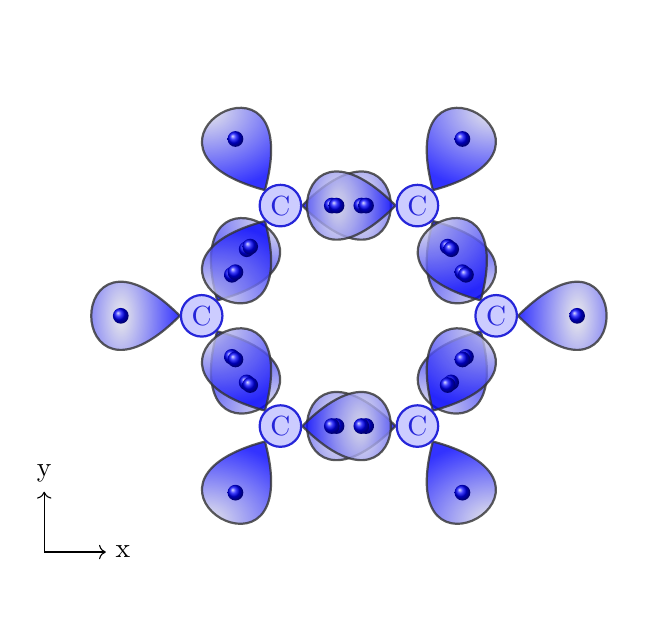
\begin{tikzpicture}
				\node (x) at (-1,-3) {x};
				\node (y) at (-2,-2) {y};
				\draw[->] (-2,-3) -- (x);
				\draw[->] (-2,-3) -- (y);
				\satom[name=C, color=blue, pos={(0,0)}]{
					blue/60/north east/2/1,
					blue/180/west/1,
					blue/300/south east/2/1
				}
				\satom[name=C, color=blue, pos={(1,1.4)}]{
					blue/0/east/2/1,
					blue/120/north west/1,
					blue/240/south west/2/1
				}
				\satom[name=C, color=blue, pos={(2.74,1.4)}]{
					blue/60/north east/1,
					blue/180/west/2/1,
					blue/300/south east/2/1
				}
				\satom[name=C, color=blue, pos={(3.74,0)}]{
					blue/0/east/1,
					blue/120/north west/2/1,
					blue/240/south west/2/1
				}
				\satom[name=C, color=blue, pos={(2.74,-1.4)}]{
					blue/60/north east/2/1,
					blue/180/west/2/1,
					blue/300/south east/1
				}
				\satom[name=C, color=blue, pos={(1,-1.4)}]{
					blue/0/east/2/1,
					blue/120/north west/2/1,
					blue/240/south west/1
				}
			\end{tikzpicture}}
		\caption{Carbon atoms in a hexagonal lattice are \(sp^2\) hybridised in the (\(x,y\))-plane.}\label{sp2}
	\end{subfigure}
	\caption{Benzene ring and its \(sp^2\) hybradised orbitals.}\label{Benz}
\end{figure}
This hybridisation lock all but one valence electron for the carbon atoms. These electrons exists in a p-orbital in the \(z\)-direction.
\cref{p} shows the valence orbitals of carbon.
\begin{figure}[H]
	\begin{center}
		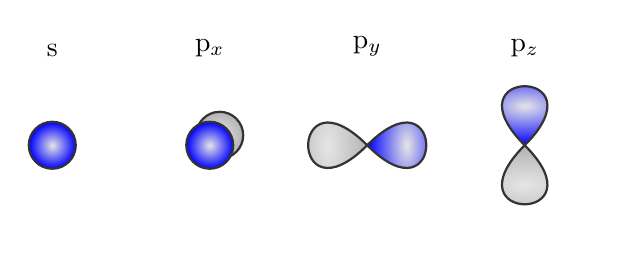
\begin{tikzpicture}
			\orbital[pos = {(0,3)}] {s}
			\node[above] at (0,4) {s};
			\orbital[pos = {(2,3)}]{px}
			\node[above] at (2,4) {p$_x$};
			\orbital[pos = {(4,3)}]{py}
			\node[above] at (4,4) {p$_y$};
			\orbital[pos = {(6,3)}]{pz}
			\node[above] at (6,4) {p$_z$};
		\end{tikzpicture}
		\caption{The valence orbitals of carbon.}
		\label{p}
	\end{center}
\end{figure}
The last electron in the p\(_z\) orbital does not mix with the tightly bound s, p\(_x\) and p\(_y\) electrons and moves freely. Thus these electrons have higher energies compared to the \(sp^2\) electrons and occupy states at the Fermi level. These electrons dominates transport in the graphene lattice. The p\(_z\) orbital is also known as the \(\pi\)-orbital and as such the electron lying there is called a \(\pi\)-electron. Through a carbon lattice the \(\pi\)-electrons will travel through \(\pi\)-orbitals. For a benzene ring the \(\pi\)-electrons at the highest occupied molecular state will travel through the p\(_\pi\)-orbitals switching sign as they travel as shown in \cref{sign}.
\begin{figure}[H]
	\begin{center}
		\pgfdeclarelayer{background}
		\pgfdeclarelayer{middle}
		\pgfdeclarelayer{foreground}
		\pgfsetlayers{background,middle,main,foreground}
		\begin{tikzpicture}
			\begin{pgfonlayer}{background}
				\orbital[pos = {(6,6)}]{-pz}
				\node[above] at (6,7) {-p$_\pi$};
				\orbital[pos = {(4,6)}]{pz}
				\node[above] at (4,7) {p$_\pi$};
				\draw[dashed, very thick] (6,6) -- (4,6);
				\draw[dashed, very thick] (7,4.73) -- (6,6);
				\draw[dashed, very thick] (4,6) -- (3,4.73);
			\end{pgfonlayer}
			\orbital[pos = {(7,4.73)}]{pz}
			\node[above] at (7,5.73) {p$_\pi$};
			\orbital[pos = {(3,4.73)}]{-pz}
			\node[above] at (3,5.73) {-p$_\pi$};
			\begin{pgfonlayer}{foreground}
				\orbital[pos = {(4,3.46)}]{pz}
				\node[above] at (4,4.46) {p$_\pi$};
				\orbital[pos = {(6,3.46)}]{-pz}
				\node[above] at (6,4.46) {-p$_\pi$};
				\draw[dashed, very thick] (4,3.46) -- (6,3.46);
			\end{pgfonlayer}
			\draw[dashed, very thick] (6,3.46) -- (7,4.73);
			\draw[dashed, very thick] (3,4.73) -- (4,3.46);
		\end{tikzpicture}
		\caption{When jumping from one carbon atom to another, the \(\pi\)-electron goes between p\(_\pi\)-orbitals. Such a jump is described by two matrix elements in the system's Hamiltonian.}
		\label{sign}
	\end{center}
\end{figure}
\subsection{Tight-binding}\label{tbtheory}
Now that the transport carrying electrons are defined the next step is describing the transport itself. For this purpose we employ the \textit{tight-binding} approximation. In this approximation the electrons are considered being tightly bound to the atoms. Contrary to a free electron gas approximation, the electrons does not spend time in between orbitals, but jump from orbital in atom \(a\) to orbital in atom \(b\). The Hamiltonian is represented as a matrix of hopping elements for a collection of neighbouring atomic orbitals, i.e. molecular orbitals, as well as the energy contained within each orbital (which will be addressed later on). This can be done by describing the orbitals as a Linear Combination of Atomic Orbitals (LCAO). The solution to the Schrödinger equation is then:
\begin{align}
	\Psi_{\mathrm{MO}} = \sum_{\alpha,R}c_{\alpha,R}\phi_{\alpha}(R)
\end{align}
where \(\phi_{\alpha}(R)\) is an atomic orbital at position \(R\), with \(\alpha\) denoting the valence of the orbital (\(2s,2p_x,2p_y,2p_z\)). In electron transport the states close to the Fermi level is of interest. These are namely the highest occupied molecular orbitals (HOMO), or the lowest unoccupied molecular orbitals (LUMO). As stated earlier only the \(\pi\)-electrons is then of interest.
The electrons' motion can be described with the hopping matrix of elements:
\begin{align}
	V_{pp\pi} = \bra{\phi_{\pi}(1)}\hat{H}\ket{\phi_{\pi}(2)}\label{V}
\end{align}
Physically this means that there is a potential between the \(\pi\) orbitals of neighbouring atoms \(1\) and \(2\). In our tight-binding approximation we consider only hop between nearest neighbours. The element
\begin{align}
	\epsilon_0 = \bra{\phi_{\pi}(1)}\hat{H}\ket{\phi_{\pi}(1)}
\end{align}
is the average energy of the electron on atom \(1\) and, it is common to define the hopping energy relative to this, i.e. \(\epsilon_0 = 0\).
If the atoms or their environment differs, so does the on-site potential.\newline
\cref{benzex} contains an illuminating example of how the tight-binding approximation can be used to describe simple carbon systems.

\section{Hamiltonian for periodic systems}\label{hamilsec}
%!TEX root = ../Main.tex
 In the following sections, the focus will be to present and explain how to calculate band structures, local density of states and transmission, through \textit{python}-programming, using Tight Binding approximation for any periodic structure. For simplicity, all initial examples and calculations will be done on a simple system, to make sure the different steps are easy to follow. The system can be seen in \cref{pointplot}.
\subsection{Creating the on-site Hamiltonian and hopping matrices}
The first and most essential parts needed for calculations is the \textit{on-site} Hamiltonian \(\mathbf{h_0}\) and the \textit{hopping} matrices \(\mathbf{V},\ \mathbf{V}^{\dagger}\). The starting point is a matrix, containing set of coordinates \(x_0,y_0,z_0\), representing atom positions  and a set of unit vectors \(\mathbf{u}_x, \ \mathbf{u}_y, \ \mathbf{u}_z\). The unit vectors will be the basis of the unit cell containing all atom coordinates. From now on, only the x and y coordinates will be considered as graphene is considered purely a 2D material.
\begin{figure}[h]
	\centering
	\begin{subfigure}[b]{0.45\textwidth}
		\includegraphics[width=\textwidth]{Figures/pointplot.eps}
		\caption{Figure showing the simple system. Every atom in the unit cell has an index, here from 0 to 7. The blue and red colours mark the left and right contacts of the system.}
		\label{pointplot}
	\end{subfigure}
	~ %add desired spacing between images, e. g. ~, \quad, \qquad, \hfill etc.
	%(or a blank line to force the subfigure onto a new line)
	\begin{subfigure}[b]{0.45\textwidth}
		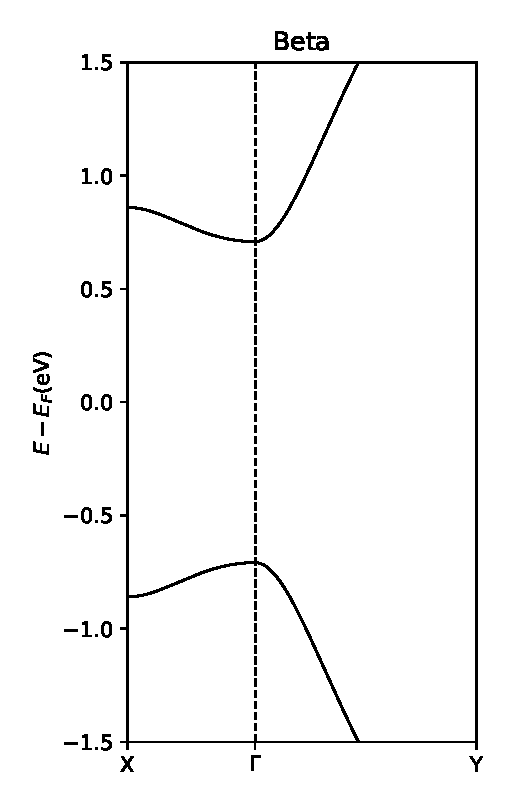
\includegraphics[width=0.7\textwidth]{Figures/BetaBandstructures.eps}
		\caption{Figure showing the band structure of the simple system.}
		\label{bandssimple}
	\end{subfigure}
	\vskip\baselineskip %add desired spacing between images, e. g. ~, \quad, \qquad, \hfill etc.
	%(or a blank line to force the subfigure onto a new line)
	\begin{subfigure}[b]{0.45\textwidth}
		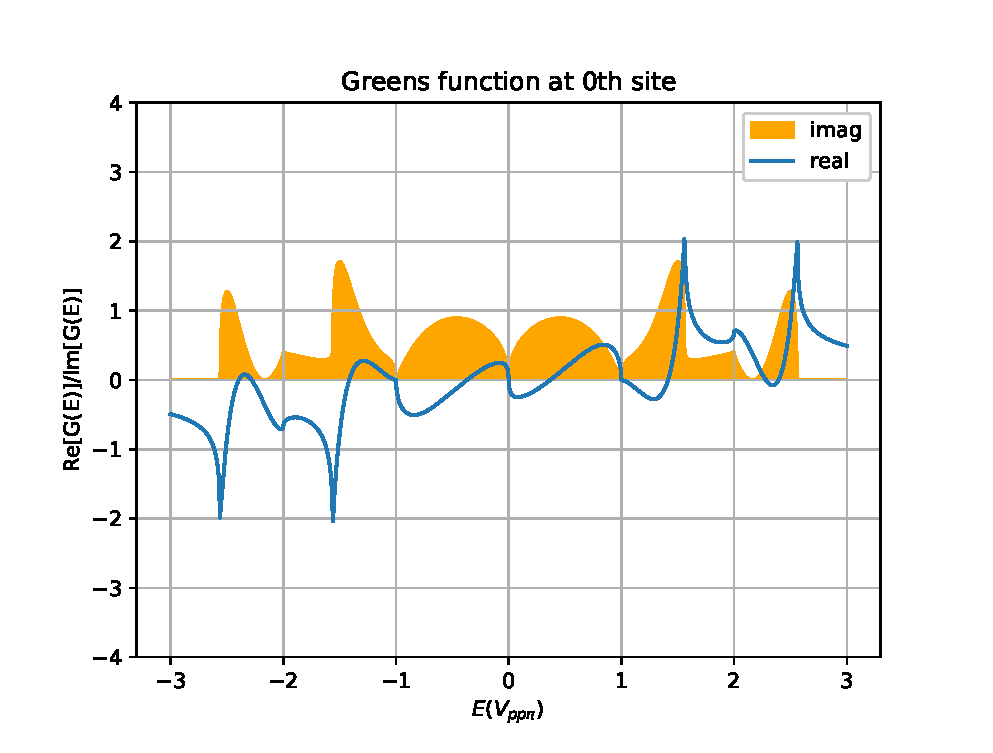
\includegraphics[width=\textwidth]{Figures/BetaimrealTE.eps}
		\caption{A plot showing the real and imaginary part of Green's function at the zeroth site resulting from the recursion routine on the simple system. Note that the yellow imaginary part is the representation of the local density of states.}
		\label{LDOSsimple}
	\end{subfigure}
	~
	\begin{subfigure}[b]{0.45\textwidth}
		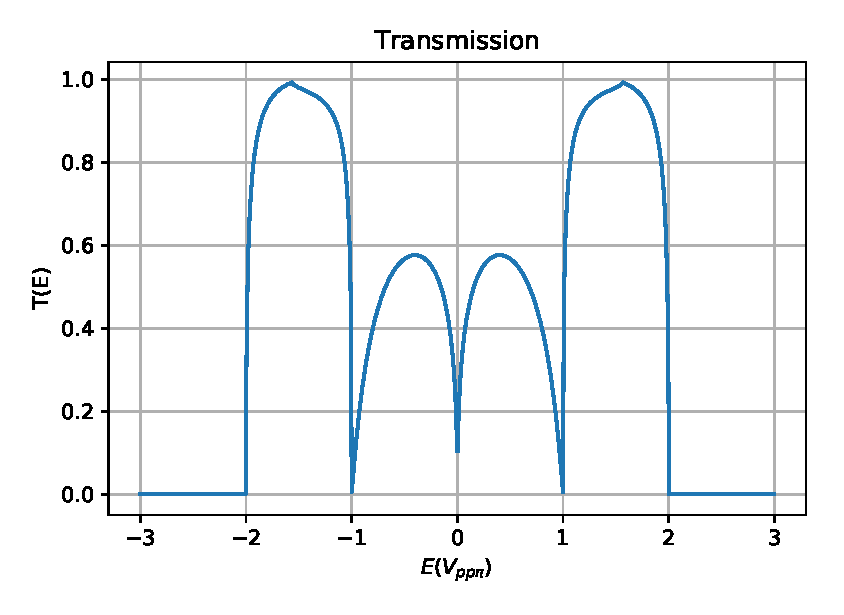
\includegraphics[width=\textwidth]{Figures/BetaTE.eps}
		\caption{\vspace{-4\baselineskip}Figure showing the resulting transmission through the simple system}
		\label{Transsimple}
	\end{subfigure}
	\caption{Figure of the different calculations executed on the simple system, using the developed scripts. }\label{eksamplefigure}
\end{figure}
The on-site Hamiltonian represents the interaction of atoms within the unit cell and the hopping matrices represents the interaction of atoms between periodically repeated unit cells. 
In \cref{atomrepfig} a visual representation of NPG with periodically repeated unit cells can be seen. For the rest of the report, the on-site Hamiltonian will all ways be the centre cell while the hopping matrices will be the cells surrounding the on-site Hamiltonian (See \cref{repfig} for a generalised visual representation of the concept). \\
In practice, the scenario is that only a data set of coordinates given from scratch. The first step is to get the on-site Hamiltonian. As mentioned the on-site Hamiltonian represents the interaction of atoms within the unit cell. The approach is then to find the atoms which interact. The interaction is based on the inter-atomic distance between atoms, so naturally one wants to find the distance between all atoms in the unit cell. To do this a subtraction of all possible combinations of two sets of atom coordinates must be done. Then taking the norm of all individual results to get the distance. A function called \textit{Onsite} have been developed to do just this. In \cref{npouter} the function can be seen.
\im{Listings/Functions.py}{31}{38}. 
\vspace{-1\baselineskip}
\captionof{listing}{The outer operator in numpy is manifested as two nested loops. On lines xx-xx each atomic distance is calculated. Line xx replaces all nearest neighbour distances with an input potential, leaving the rest as zero. Lastly the diagonal is subtracted from the matrix.\label{npouter}}\vspace{\baselineskip}
The function produces a matrix which contain all distances between all atoms in the unit cell. The Tight Binding model dictates that only atoms with a specific inter-atomic distance interact. Therefore the function has implemented a threshold (\cref{npouter} line xx) to determine whether a given distance is too great for interaction or small enough for interaction. All distances above the threshold will be changed to a 0-element in the on-site Hamiltonian matrix, representing zero interaction and all distances below the threshold will be changed to 1 to represent interaction between atoms. Finally The on-site Hamiltonian is multiplied with a on-site potential (scalar). The on-site potential \(V_{pp\pi}\) differs depending on the system. Now the on-site Hamiltonian is complete and the product is a matrix containing 0's and 1's to represent interaction between atoms in a unit cell. \\
Moving on to the hopping matrices one first has to realise that the interactions are happening in a 2D plane. This has to be kept in mind when describing interaction between unit cells repeated in all directions in the plane. Effectively this means that six hopping matrices should be created. One in the x-direction, one in the y-direction, one in the xy-direction and their hermitian conjugates. Graphically this corresponds to a structure of this kind:
\begin{figure}[H]
	\centering
	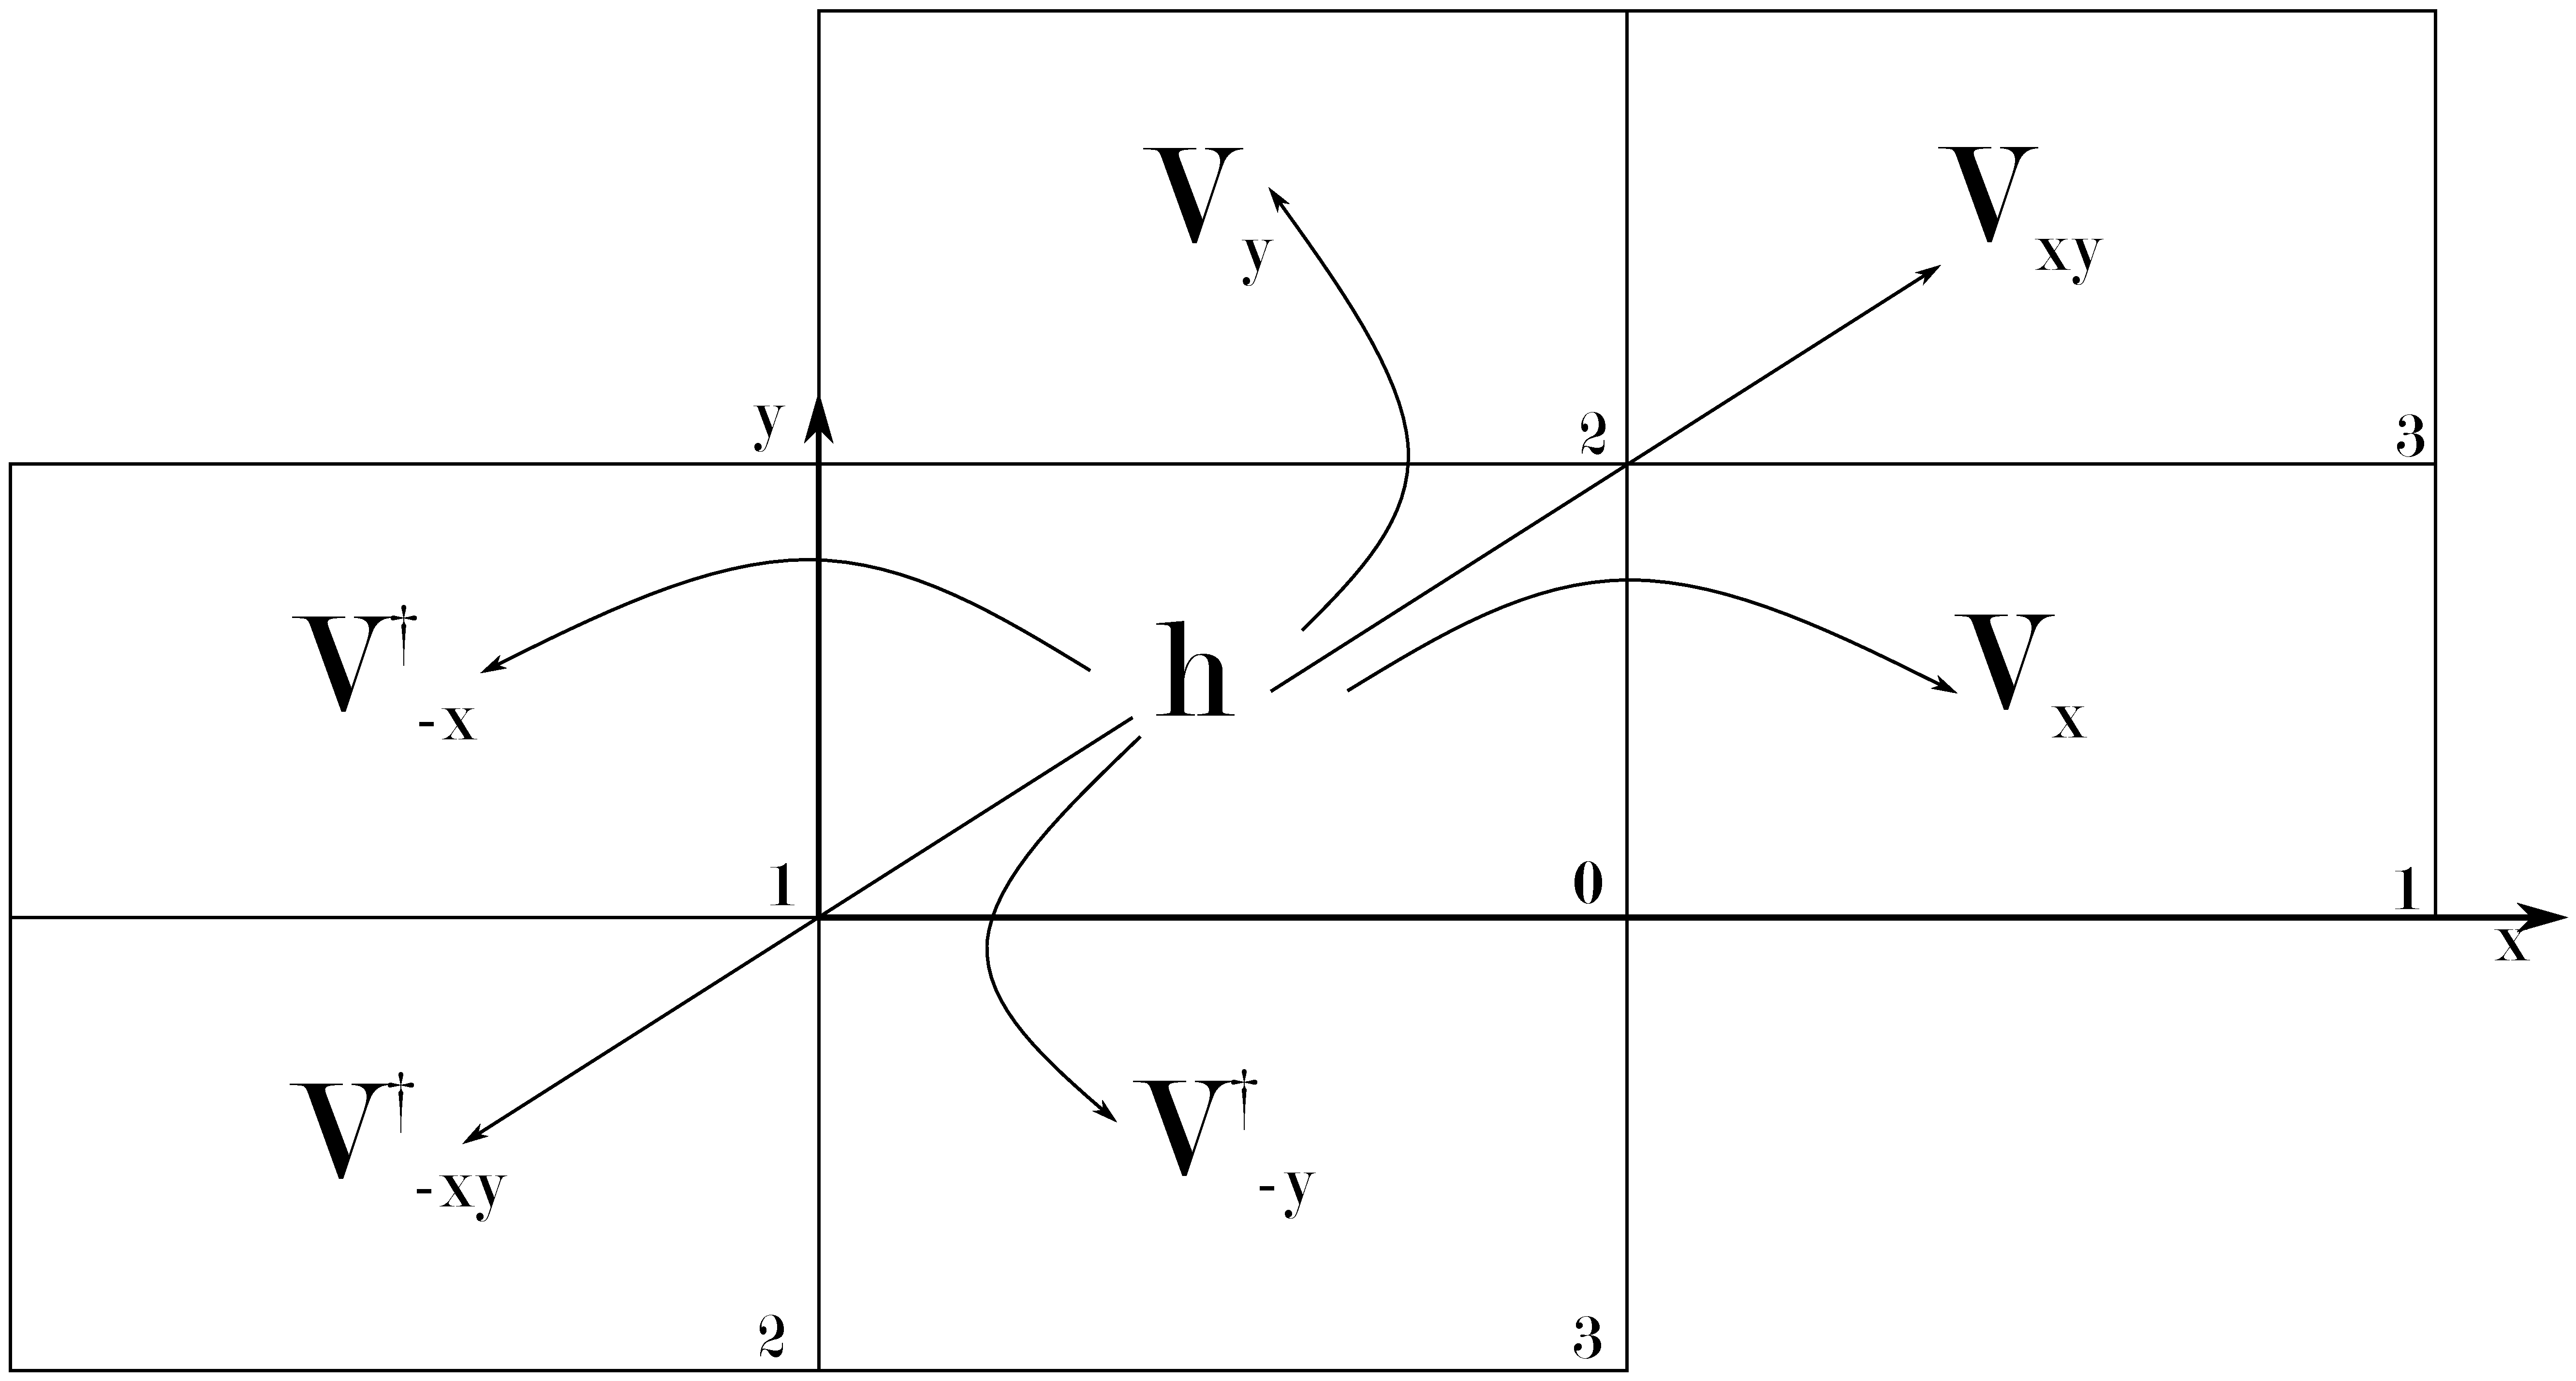
\includegraphics[width = 0.7\textwidth]{Figures/repfig.eps}
	\caption{Representative figure of how the on-site Hamiltonian along with its hopping matrices are structured}
	\label{repfig}
\end{figure}
In practice this is done by shifting the original \(x_0,y_0\) coordinates by the given unit vectors \(\mathbf{u}_x,\mathbf{u}_y\). By addition of the unit vectors to the original coordinate matrix one can get three new coordinate matrices \(\mathbf{xy}_{shift-x}=x_0,y_0 + \mathbf{u}_x\), \(\mathbf{xy}_{shift-y}=x_0,y_0 + \mathbf{u}_y\) and \(\mathbf{xy}_{shift-xy}=x_0,y_0 + \mathbf{u}_x+\mathbf{u}_y\). With these three matrices what follows is basically the same method used to get the on-site Hamiltonian. The only difference being that it will be distances between atoms in the on-site Hamiltonian and the shifted matrices respectively. That way it is the distance, and thus the interaction, between the on-site Hamiltonian and the repeated unit cells that is calculated. The three resulting hopping matrices are denoted \(\vb{V}_{1x}\), \(\vb{V}_{2y}\) and \(\vb{V}_{3xy}\). They represent interaction (hopping) in the "forward" direction (left-to-right) (See \cref{repfig}). To create the hopping matrices hopping in the "backwards" (right-to-left) direction (See \cref{repfig}) one simply has to transpose the hopping matrices. These matrices are denoted with a dagger: \(\vb{V}_{1x}^{\dagger}\), \(\vb{V}_{2y}^{\dagger}\) and \(\vb{V}_{3xy}^{\dagger}\). The matrices are programmed using the developed function \textit{Hop}, which can be seen in \cref{appfigs}, \cref{hopfunc}. To show how the on-site Hamiltonian and the hopping matrices look, see \cref{matrixmap} for a figure of the resulting matrix-maps from calculation on the small simple system. It has been stitched together like in \cref{repfig}. To see how the function running the calculation for the hopping matrices look in \cref{appfigs}, \cref{hopfunc}. 
\begin{figure}[H]
	\centering
	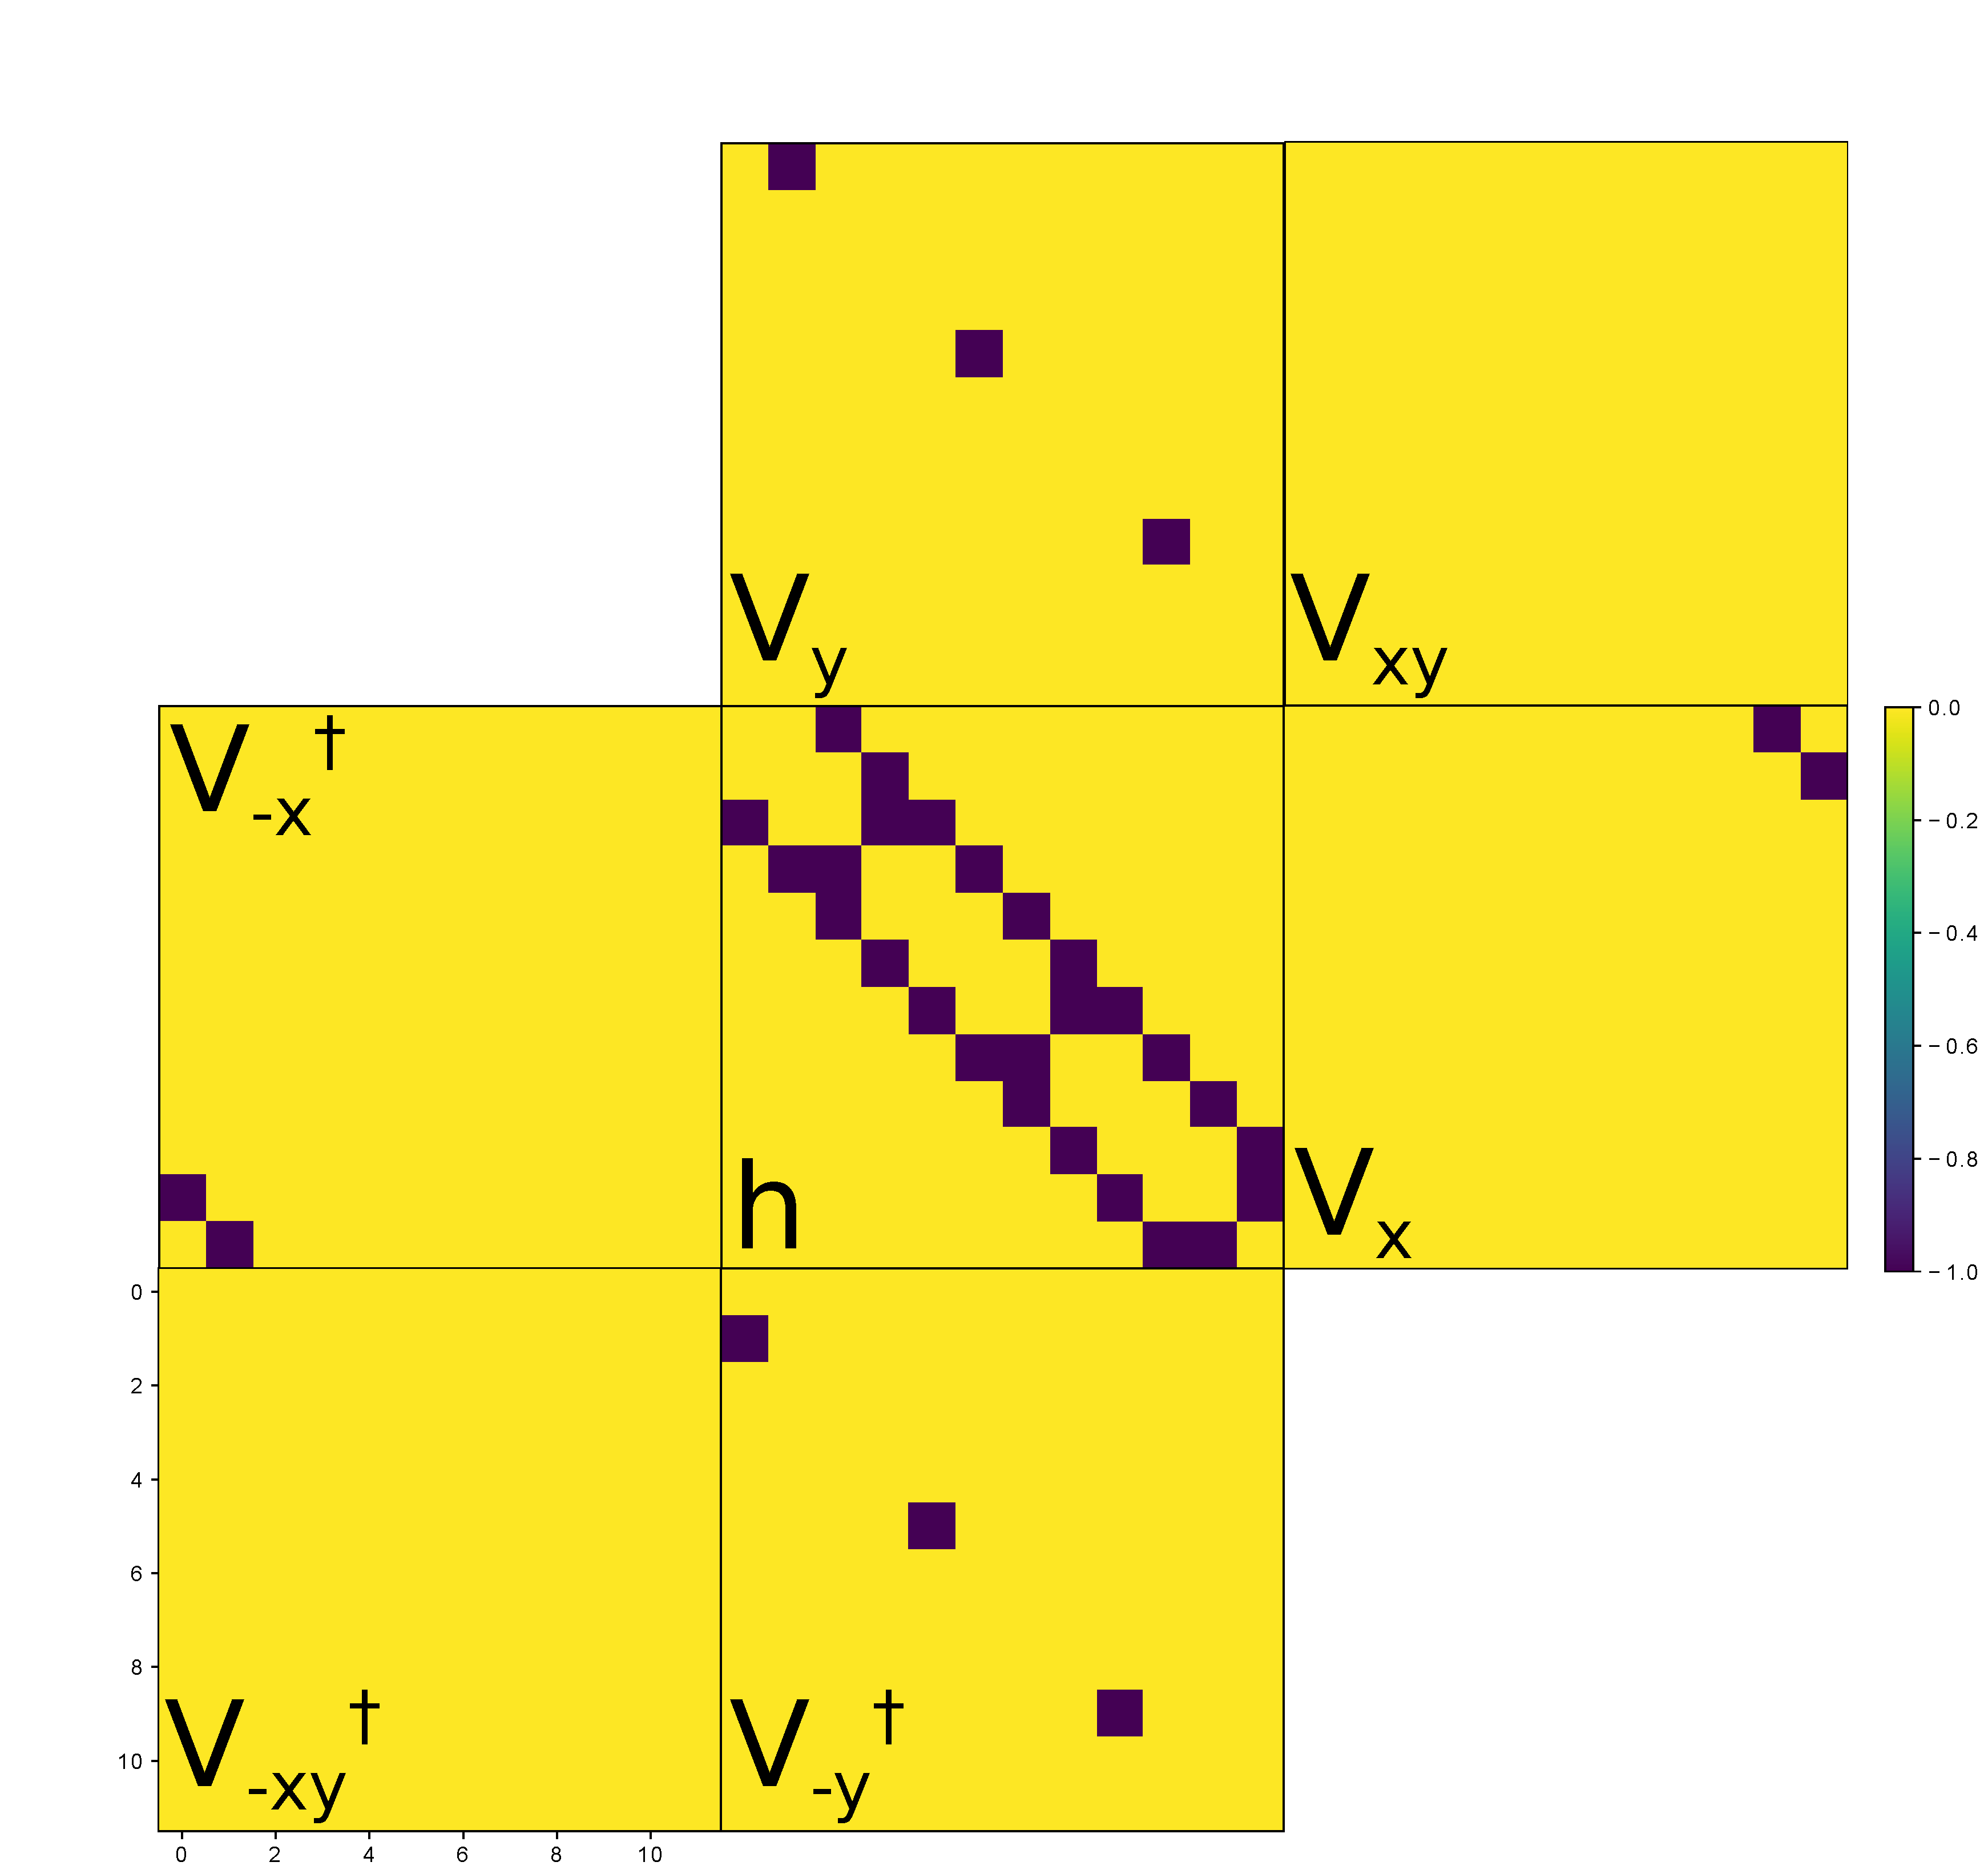
\includegraphics[width=0.7\textwidth]{Figures/stitch.eps}
	\caption{Matrix maps from calculation on an arbitrary graphene system with a unit cell of 12 atoms. The on-site Hamiltonian along with all its hopping matrices are stitched together like in figure \cref{repfig}. All the dark spots represent a hopping of an electron to its nearest neighbour i.e. a 1 element and yellow represents a 0 element}
	\label{matrixmap}
\end{figure}
\subsection{Defining the full Hamiltonian and solving the Schr\"{o}dinger equation}\label{FullHam}
Now that the on-site Hamiltonian along with its hopping matrices have been created, the next step is to create the full Hamiltonian in order to solve the Schr\"{o}dinger equation for the system as a whole. This is an eigen-value/vector problem. The Schr\"{o}dinger equation needs to be solved to get the eigen energies for the system as they will be used to produce band structure plots later on. In essence the full Hamiltonian denoted \(\vb{H}\) is a sum of the on-site Hamiltonian and its corresponding hopping matrices multiplied by a complex exponential function that has the appropriate phase relative to the hopping matrix:\begin{align}\label{hamileq}
	\vb{H}(k_x,k_y) = \vb{h}_0 & + (\vb{V}_{1x}e^{-ik_x} + \vb{V}_{1x}^{\dagger}e^{ik_x}                              \\ \nonumber
	                           & + \vb{V}_{2y}e^{-ik_y} + \vb{V}_{2y}^{\dagger}e^{ik_y}                              \\
	                           & + \vb{V}_{3xy}e^{-ik_x}e^{-ik_y} + \vb{V}_{3xy}^{\dagger}e^{ik_x}e^{ik_y}) \nonumber
\end{align}Here \(k\) represents a continuous variable between 0 and \(\pi\) along the \(\dfrac{1}{x}\)- and \(\dfrac{1}{y}\)-axis in reciprocal space.
Using the full Hamiltonian, the Schrodinger equation can be solved
\begin{align}
	\vb{H}(k_x,k_y)\vb*{\phi}_{k} = \vb*{\epsilon}_n (k_x,k_y) \vb*{\phi}_k
\end{align}
Where \(\vb*{\phi}_k\) is the and \(\vb*{\epsilon}(k_x,k_y)\) is the eigen energies. \\
In practice this is done by defining a function, here called \textit{Hkay}, that takes the on-site Hamiltonian, the hopping matrices, and \(k_{x/y}\) as inputs and outputs the eigenvalues, using numpy's \textit{numpy.linalg.eigh}. The number of eigenvalues in the output corresponds to the dimension of the full Hamiltonian. In \cref{fullhamil} the code for the function is shown.
\im{Listings/Functions.py}{50}{59}
\vspace{-1\baselineskip}
\captionof{listing}{Function producing the full hamiltonian, corresponding to \cref{hamileq} the inputs x and y corresponds to the \(k_x\),\(k_y\) .\label{fullhamil}}\vspace{\baselineskip}
\subsection{Producing band structures}
%An important intrinsic information in any solid state matter is of course the band structure as it gives information about allowed electron energies at different points in the material. Specifically for NPG, the band structure may be used to track the changes of electronic transport upon changing the bridges connecting GNR's within NPG.
In order to calculate and visualise the band structure of the simple system, one need to define the full Hamiltonian \(\mathbf{H}\) in two directions. When working with band structures and periodic systems it is common to note points in space with respect to the \textit{Brillouin Zone} which is a primitive cell in reciprocal space. Therefor 
a continuous variable \(k\) is introduced. it extends in two directions in (\(-k_{x}\)) and (\(k_{y}\)), which correspond to lengths between the symmetry points \(X\), \(\Gamma\) and \(Y\) in the Brillouin zone. Here \(\Gamma\) is the origin \((0,0)\). Practically this corresponds to making two plots, one for each pair of symmetry points. The y-values in each plot correspond to the eigenvalues obtained by the \textit{Hkay} function described in \cref{FullHam}. The number of eigen energies, and effectively the number of bands in the plot is dictated by the dimension of the Hamiltonian. \(n\times n\)-matrix \(\rightarrow\) \textit{n} eigen energies (bands). However plots produced in this report will only show a few of these bands in a small energy range. In the case of the simple system, the full Hamiltonian for obtaining the eigen energies that corresponds to directions \(X\) and \(Y\) are:\begin{align}
	X: \ \vb{H}_{X} = \vb{h}_0 + (\vb{V}_{1x}e^{ik_x} + \vb{V}_{1x}^{\dagger}e^{-ik_x} + \vb{V}_{2y} + \vb{V}_{2y}^{\dagger} + \vb{V}_{3xy}e^{ik_x} + \vb{V}_{3xy}^{\dagger}e^{-ik_x}) \\
	Y: \ \vb{H}_{Y} = \vb{h}_0 + (\vb{V}_{1x} + \vb{V}_{1x}^{\dagger} + \vb{V}_{2y}e^{-ik_y} + \vb{V}_{2y}^{\dagger}e^{ik_y} + \vb{V}_{3xy}e^{-ik_y} + \vb{V}_{3xy}^{\dagger}e^{ik_y})
\end{align}Using the eigenvalues as y-values in the two plots, putting the two plots together will yield a final plot of the band structure shown in \cref{bandssimple}. 



\section{Greens Functions, Self Energy and the Recursion Routine}\label{greensec}
In order to calculate the transport of electrons in NPG one must obtain the Green's functions and self energies related to the unit cells of the system. To do so, a recursion algorithm must be implemented as calculations become too costly for the system, even if it is small. Especially the inversion of matrices required to obtain the Green's function can be very demanding computationally, when the system contains a lot of atoms. The recursion algorithm reduces the size of the system and thereby the amount of computational time required to obtain both the first cell Green's function, the Green's function within the chain (of repeated unit cells) sometimes called \(\mathbf{G}_{bulk}\) as well as the self energies related to those Green's functions. The recursion works by utilising that one can remove every second cell in an infinite chain of cells. As the chain originally was infinite, removing every second cell will just yield a new infinite chain. Every cell has with it, its hopping matrices and hamiltonian. The removal of every second cell is iterated, changing the effective interaction between the cells and thus the hopping matrices as well as the hamiltonians of the system. In the end the recursion algorithm produces re-normalised hamiltonians and hopping matrices, which can be used to obtain the Green's functions and self energies. 
\subsection{Obtaining first cell self energy and Green's function for a simple four-atom system}\label{recursionroutinesec}
For simplicity and in order to check whether the routine would yield the results expected, the starting point is a simple system containing only 4 atoms in the unit cell. The idea is to make a function that takes in an energy, a hamiltonian (alternatively two in case there is a special site in the molecule) and a hopping matrix as arguments and outputs the Green's function at the zeroth site as well as the self energies going left and right. Firstly all the necessary variables are defined. The first of these consists of a complex number matrix which has the value \(E + i\eta\) in the diagonal and dimension identical to that of the hamiltonian given as argument. Here \(E\) is the energy which the function takes as an argument and \(\eta\) is a small number (in this specific case \(1\times10^{-6}\)). Note that \(\eta\) should not be made too small as it will yield incorrect results. The rest of the variables are the hamiltonian, hopping matrices and Green's function. They are defined as: \(a0 = V^{\dagger}, \ b0 = V, \ e0_{s} = h, \ e_{0} = h, \ g0 = (z-e0)^{-1}\). Note that the hamiltonian \(h\), in this specific case, is the same for both \(e0_{s}\) and \(e0\) as the zeroth cell is identical to those of the rest of the molecule. Now that the variables is defined, the actual recursion can begin. As the recursion is an algorithm that runs for an arbitrary amount of iterations, a while loop is chosen to run the iterations until a threshold has been reached. In \cref{recursfunc1} the code for the routine is shown. Line 64-70 is the listing of variables, 71-78 is the while loop with the matrix multiplication, 80-84 is the redefinition of new variables in terms of the old and 86-89 is the definition of the outputs as per \cref{outputs}.\\
\noindent
\begin{listing}
    \begin{minipage}[b]{.40\textwidth}
        \inputminted[bgcolor=Black, breaklines, breakanywhere, linenos=true, python3=true, firstline=64, lastline=79]{python}{Listings/Functions.py}
    \end{minipage}
\end{listing}
\begin{listing}
    \begin{minipage}[b]{.40\textwidth}
        \inputminted[bgcolor=Black, breaklines, breakanywhere, linenos=true, python3=true, firstline=80, lastline=91]{python}{Listings/Functions.py}
    \end{minipage}
\end{listing}The threshold is defined as the absolute maximum value in the hopping matrix \(a0\) approaches zero. In this specific case it was set to \(1\times10^{-8} \). Within this while loop a range matrix multiplications are computed. These constitutes the actual recursion and their order are of big importance for a correct result. Notice, however, that the code (\cref{recurfunc}) contains intermediate products of \(a0, b0\) and \(g0\). This is for run time optimisation. Following is a list of these matrix multiplications: 
\begin{align*}
a1 &= a0\ g0\ a0\\ 
b1 &= b0\ g0\ b0\\ 
e1 &= e0 + a0\ g0\ b0 + b0\ g0\ a0 \\
e1_{s} &= e0_{s} + a0\ g0\ b0 \\ 
g1 &= (z - e1)^{-1} 
\end{align*}
As stated above in the equations, the matrix product are defined as new variables with a \(+1\) variable name. This is all very well but the while loop would stop here because of the definition of new variables. It is therefore necessary to redefine the new variables in terms of the old ones (f.ex. \(a0 = a1\)) (see \cref{recurfunc2}) an as such the while loop will continue until the threshold has been reached. For the rest of the function the only thing left to do is to define the self energies and the first cell Green's function using the variables obtained from the while loop. These are simply given as: 
\begin{align}\label{outputs}
    \mathbf{\Sigma}_R &= e_s - h \\ \nonumber
    \mathbf{\Sigma}_L &= e - h - \mathbf{\Sigma}_R \\ \nonumber
    \mathbf{G00} &= (z - e_s)^{-1}
\end{align}
Where \(e_s\) and \(e\) are the resulting matrices from the while loop (\(e0_s, e0\)). The first cell Green's function as well as the self energies has now been obtained by recursion. 
\subsection{Plotting the real and imaginary part of the first cell Green's function}
As a good way to check whether the recursion routine has been implemented successfully, the real and imaginary part of the Green's function can be plotted. With a relatively simple approach, the Green's function can be obtained as a function of energy, using a \textit{for loop}, looping over a range of energies which is then used as input in the function \cref{recursionfunc} (see \cref{plotcode}):
\begin{listing}[ht]
    \im{Listings/SelfEnergyByRecursion.py}{64}{68}
    \caption{Code showing the loop which produces the Green's function (or y) values for a range of energies used in the plot.}
    \label{plotcode}
\end{listing}
The output from this loop will be the real and imaginary y-values for the plot. These will have to be sorted to imaginary and real parts before plotting. The x-values will just be the energy range used for the loop. The imaginary part of the Green's function is especially important as it represents the local density of states LDOS. Following is the plot of the real and imaginary part of the first cell Green's function obtained by the recursion routine for the simple four atom unit cell described in \cref{recursionroutinesec}. In \cref{imrealplot} a plot of the imaginary and real part of the resulting Green's function can be seen. 
\begin{figure}
    \centering
    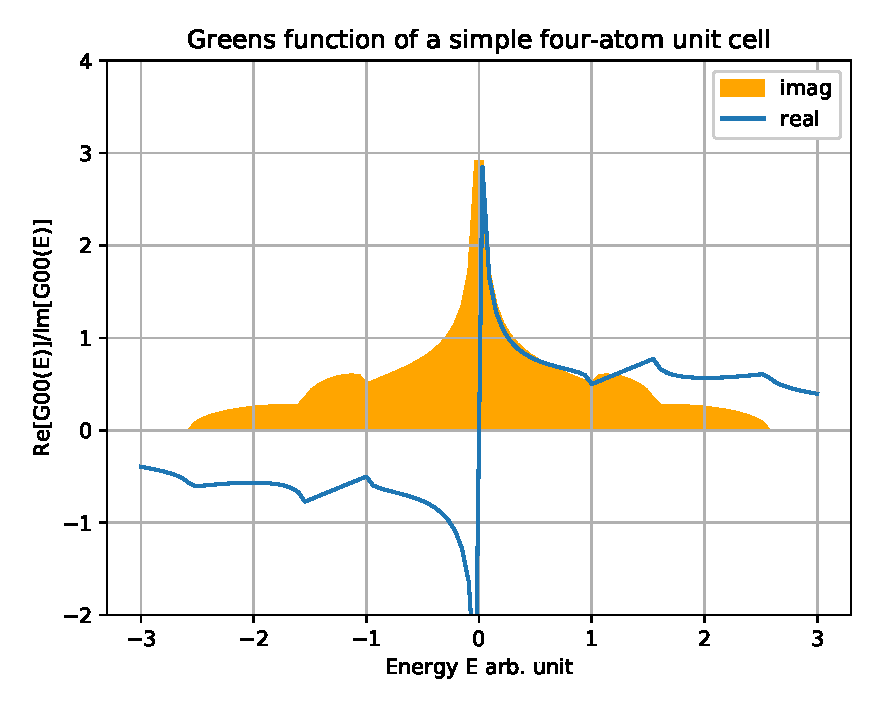
\includegraphics[width = 0.5\textwidth]{Figures/imrealplot.eps}
    \caption{A plot showing the real and imaginary part of the first cell Green's function resulting from the recursion routine on the simple system. Note that the yellow imaginary part is the representation of the density of states.}
    \label{imrealplot}
\end{figure}

\section{Transmission Routine}\label{transec}
%!TEX root = ../Main.tex
The conclusion of the preliminary work revolves around the Transmission Routine. Here all the functions producing on-site hamiltonians, full hamiltonians, hopping matrices, bandstructures, self energy and Green's functions by recursion play their part in getting the transmission through the material. \textit{This part is an attempt to describe the basic theory behind transmission/transport and it is very likely to need rework, additions and editing} The transmission tells us the likelihood whether an electron will be transported trough a "device region" at different energies and thus how the "device region" affects the overall current through larger systems. This means that the system will have to be well defined before one can use the functions developed for calculation of the different parts needed for production of transmission. The "device region" contains at least one central unit cell as well as a "left" and "right" unit cell. The left and right unit cell represents the contact region of the device i.e. the two parts that connects to the "rest" of the system/molecule. It is assumed that the contacts represent a system that is made up of unit cells which can be reduced by recursion, though not necessarily identical on each side (left and right). Knowing which "blocks" the system contains and how to obtain them with the already developed functions, three main ingredients are needed to obtain the transmission through a device. The first one is the Green's function for the device region \(\mathbf{G}_D\) for which one needs the device hamiltonian \(\mathbf{H}_D\) as well as the left and right selfenergies \(\mathbf{\Sigma}_L, \ \mathbf{\Sigma}_R\). The left and right selfenergies constitutes the second ingredient and can be obtained through left and right hopping matrices as well as the left and right on-site Green's functions. The last main ingredient are \(\mathbf{\Gamma}_L,\ \mathbf{\Gamma}_R\) which are matrix operators describing the coupling between the left and right parts of hilbert space. They are called rate equations because..... The rate equation are obtained via the self energies in the following fashion: 
\begin{align}
\mathbf{\Gamma}_{L/R} = i(\mathbf{\Sigma}_{L/R} - \mathbf{\Sigma}^{\dagger}_{L/R})
\end{align}To give an overview of how the different matrices are defined in relation to a system an illustration has been made.See \cref{systemillu}. Using the Green's function, left/right self energies as well as the left/right rate matrices, the transmission, as a function of energy, can be obtained via the following equation:
\begin{align}
    T(E) = \text{Tr}[\mathbf{\Gamma}_R\mathbf{G}_D\mathbf{\Gamma}_L\mathbf{G}_D^{\dagger}](E)
\end{align}
Where Tr is the trace of the matrix product. 
\begin{figure}
    \centering
    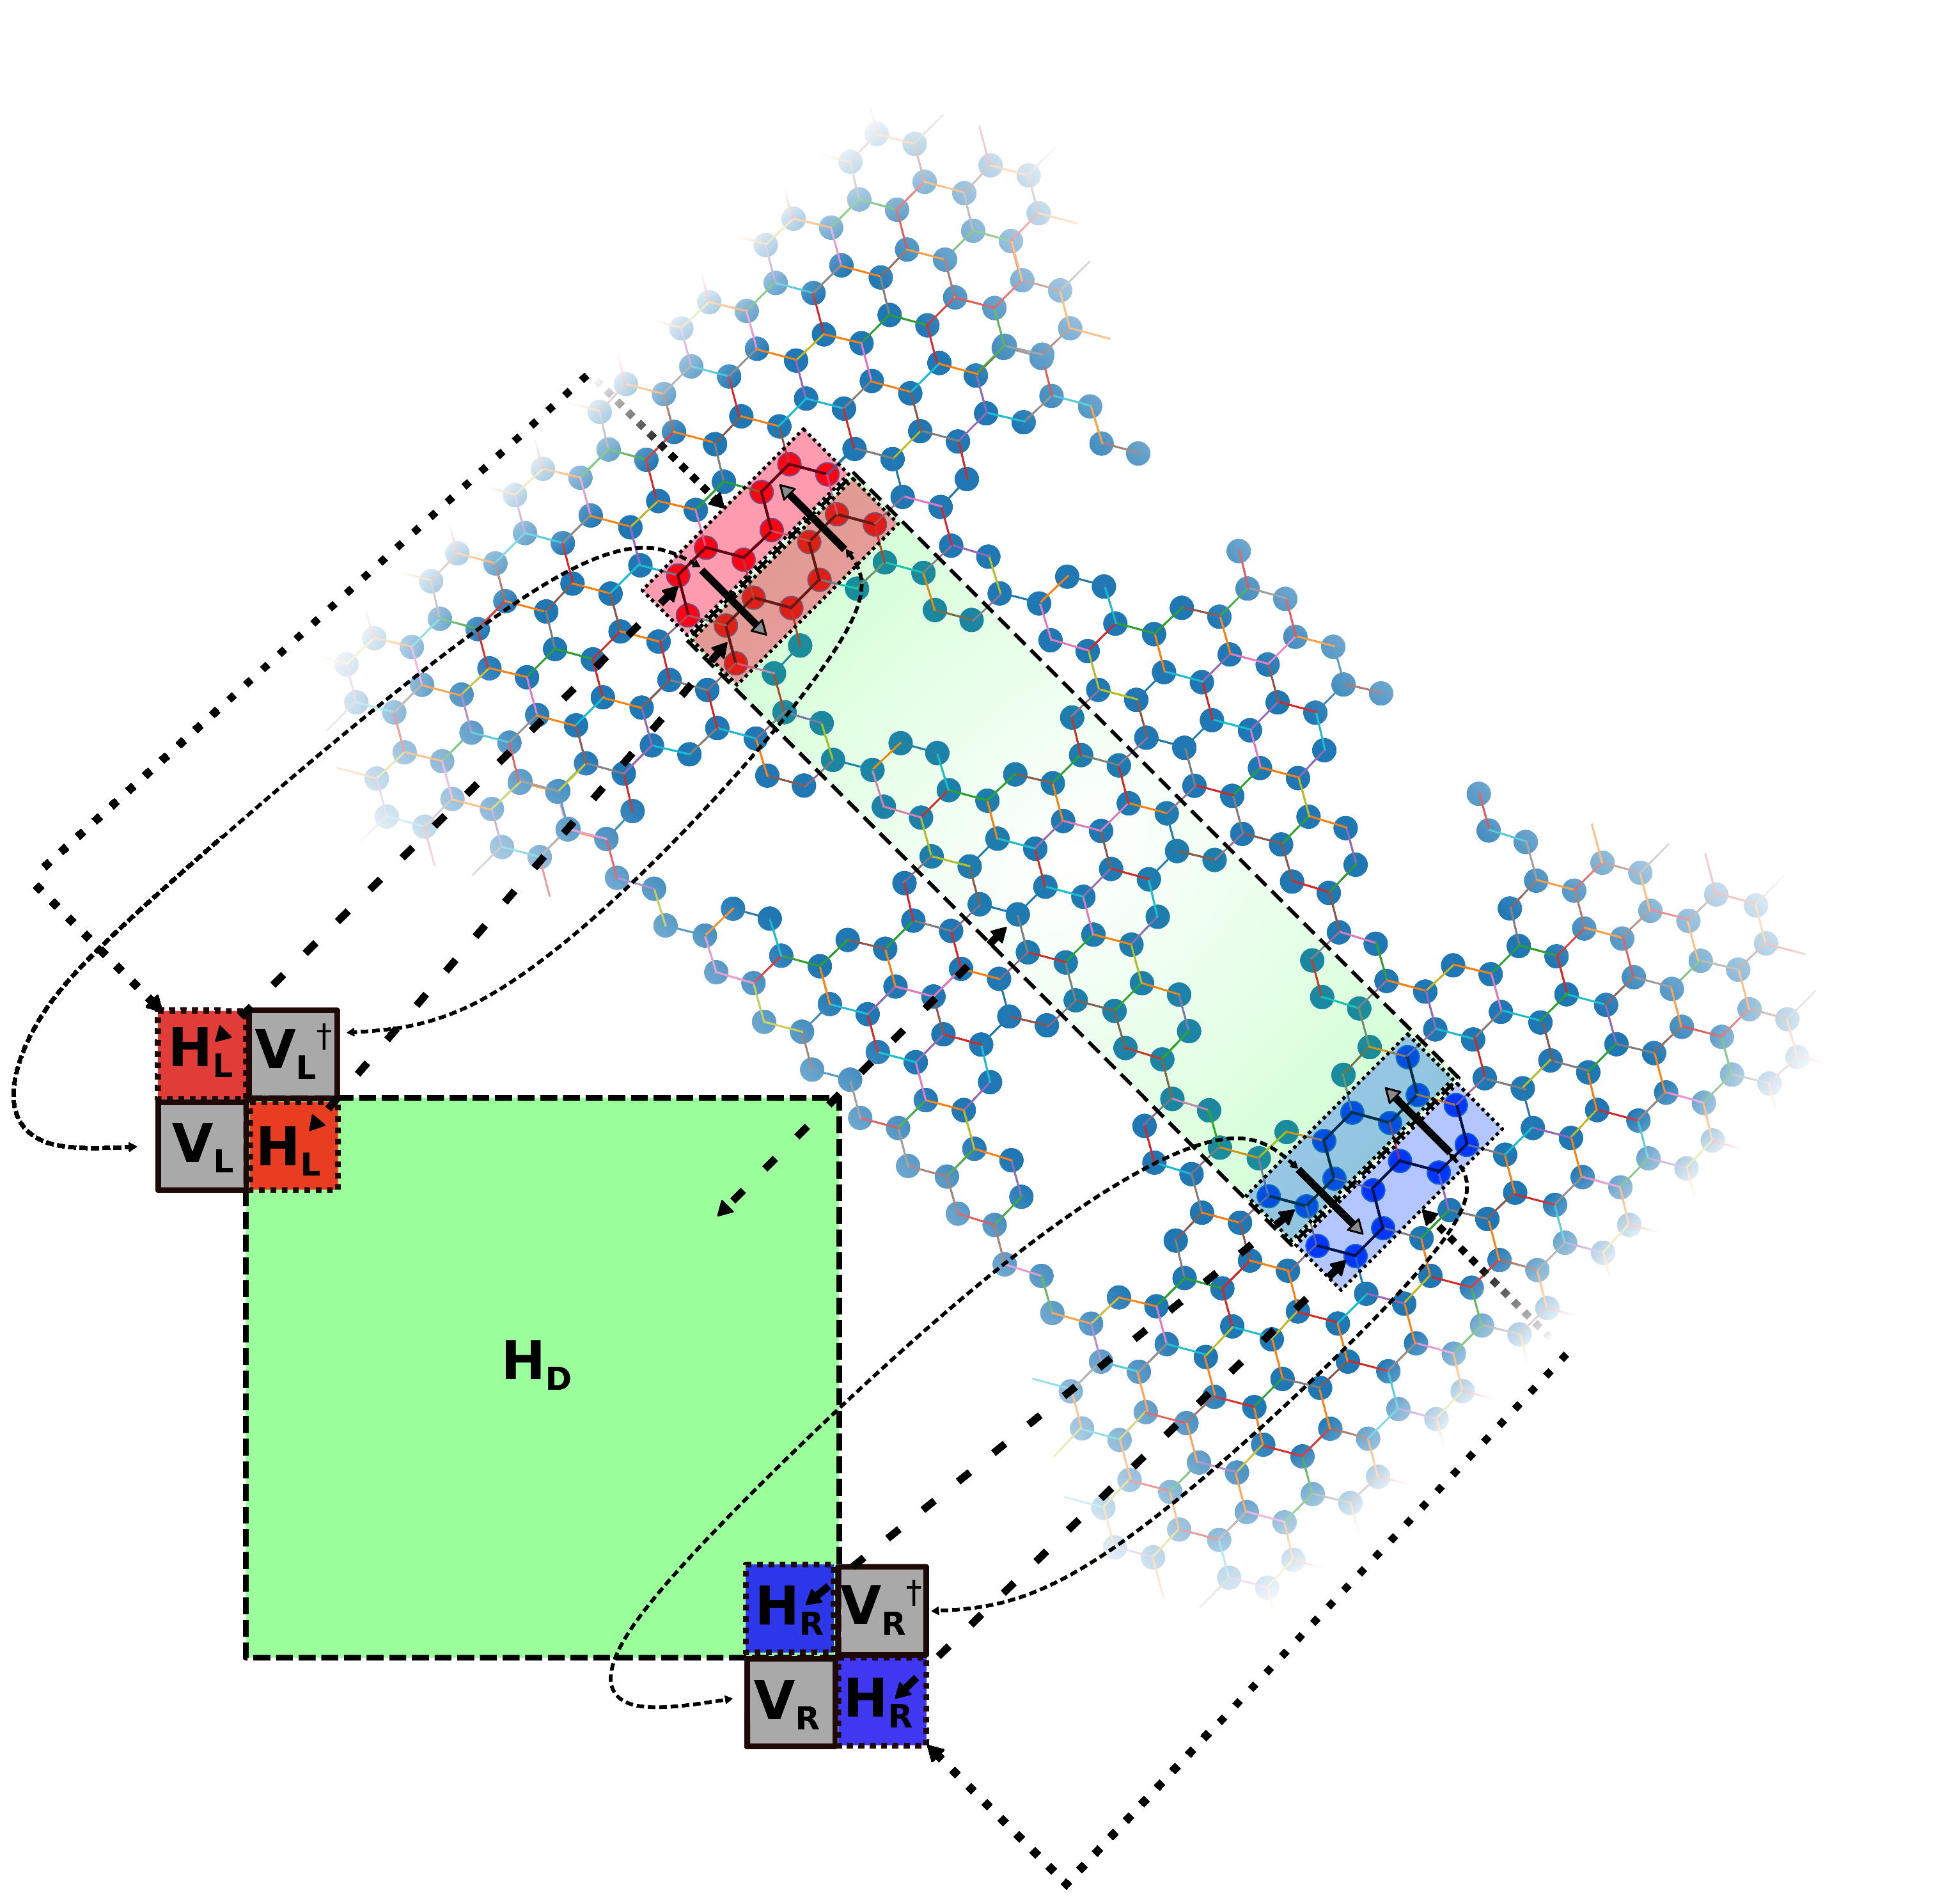
\includegraphics[width=0.9\textwidth]{Listings/illu.eps}
    \caption{Illustration showing how the different parts of the system are translated into matrix blocks. On the graphene the green box is the unit cell of the device. It includes one red and blue box which themselves are unit cells of the left and right contacts. These unit cells can be translated into hamiltonian matrices \(\textbf{H}_D, \ \textbf{H}_L,\ \textbf{H}_R\) as illustrated. Note that because the first of the left and right unit cells (red and blue) are inside the device (green region), they can be picked out of \(\textbf{H}_D\) directly and so it is not necessary to make them from scratch. The two other unit cells lying outside the device region represents what could be an infinite contact region. The contact region is therefore potentially of an infinitely bigger dimension compared to the device region, however, by recursion, this region can be collapsed into a single hamiltonian of same dimension as the one inside the device region. Finally the two fat black arrows on each side of the device represents the hopping between the device and contact region. Note that the direction of hopping corresponds to a specific hopping matrix. F.ex. left-to-right is the ordinary hopping matrix while right-to-left is its conjugate (for both left and right).}
    \label{systemillu}
\end{figure}
\subsection{Transmission in 1D a simple example}
As with the Recursion Routine, the development of this routine will be build up around a small system in order to make sure that the obtained results are as expected, thereafter generalising the routine to suit all kinds and sizes of system.


\section{Exploring functionality of GNR bridges}\label{testsec}
%!TEX root = ../Main.tex
In this section a range of tests will be conducted on different NPG structures in order to uncover the effect of manipulation of the bridges between the GNR's in the NPG. From an applied perspective, one of the main motivations is to find out how these bridges can be manipulated in order to control the current through the material. A recent study has shown how one could possibly confine current flow to a single GNR channel by manipulation of bridges between GNR's utilising \textit{Quantum Interference} effects, thus providing a solution to an important aspect in carbon-based nanocircuitry design, namely confinement of electron flow. The study was focused on the difference in effect of having \textit{meta} and \textit{para} bridges between GNR's. Meta and para bridges are essentially benzene rings oriented in two different ways (more on that in the following sections). The meta and para bridges are 'static' cases in the sense that once made, they are not responsive to any external environment. However, if the bridges are modified with oxygen they become sensitive to f.ex. hydrogenation because of oxygen's tendency to either reduce or oxidise in basic/acidic environments. Thus by hydrogenation it will be possible to tune the electrical properties of the material and make it sensitive to external environments and studies has show that hydrogenation of specific sites on nano meter scale is possible experimentally. This section will, in part, be an attempt to reproduce some of the results of the study and to see what happens when if oxygen is added to these benzene rings in the meta and para bridges as well as the effects of hydrogenation of the oxygen.  In \cref{testtable} a schematic overview of the different tests can be seen. The results from these tests will be presented in the form of band structure plots and they will be compared to band structure plots produced with DFT. Additionally a schematic overview of the different systems, showing the on-site potentials of each atom will be presented in the figures as well. Following is a section introducing meta and para NPG in detail. 
\begin{table}[ht]
\begin{tabular}{cclcll}
		\toprule
		Test no. & Meta/Para & Symmetry   & No. of species & Added species & Name  \\ \midrule
		1        & Para      & Symmetric  & 4              & Oxygen        & PS4O  \\
		2        & Para      & Symmetric  & 4              & Hydroxide     & PS4OH \\
		3        & Meta      & Symmetric  & 2              & Oxygen        & MS2O  \\
		4        & Meta      & Symmetric  & 2              & Hydroxide     & MS2OH \\
		5        & Meta      & Asymmetric & 2              & Oxygen        & MA2O  \\
		6        & Meta      & Asymmetric & 2              & Hydroxide     & MA2OH \\
		\bottomrule
	\end{tabular}
	\caption{Table showing an overview of all the structures that will be tested in this section.  How the different species will be manipulated during the tests, will be stated in plots produced for results. The code names follow the table column-wise. In \cref{appfigs}, \cref{Strucow} a collection of figures showing each scenario stated in this table.}
\label{testtable}
\end{table}
\subsection{Differences in para and meta bridges}
In broad terms the difference in the meta and para structures lies in the path an electron will travel through the benzene ring to get across the bridge. In the para bridge, the path across the aromatic ring is symmetric and so the electron will pass above or below with equal probability. Since the para bridge has three bonds in each direction across the ring, the path length in the para bridge is the same on each side (See \cref{metapara}). This will cause constructive interference of the states once the waves meet on the other side of the ring, which results in spreading in the density of states from one GNR to the next. For the meta bridge the way across the aromatic ring is not symmetric in the sense that there is two bonds across the path below and four bonds across on the path above (See \cref{metapara}). This will cause a shift by half a wavelength between the two paths and thus create destructive interference between waves meeting on the other side of the ring. The effect of this is confinement in the density of states in the GNR's. 
\begin{figure}
    \centering
    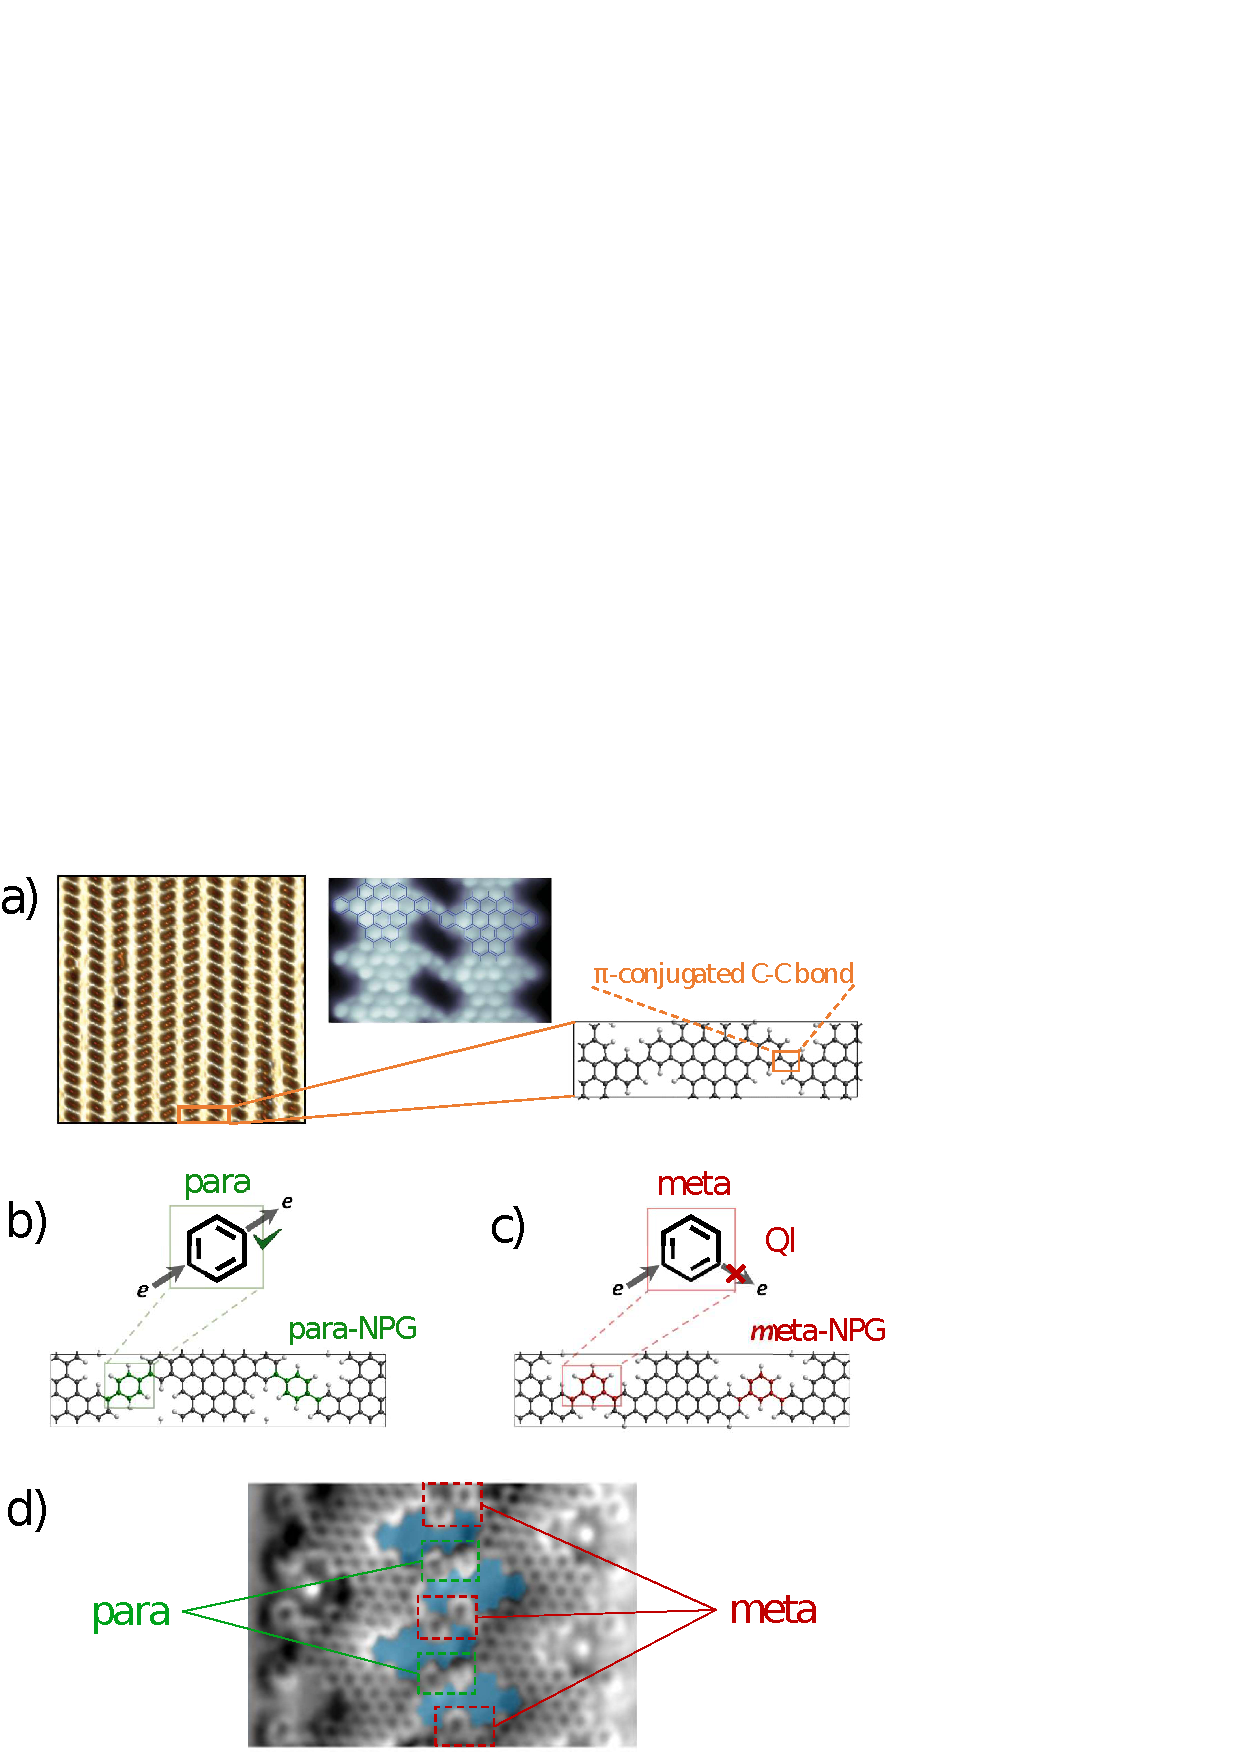
\includegraphics[width=0.5\textwidth]{Figures/Fig_1.pdf}
    \caption{Figure obtained from [cite] showing the difference of para and eta bridged both graphically and with picture}
    \label{metapara}
\end{figure}
\subsection{Tests with modified meta and para NPG}
The tests consist of three kind of manipulations. Firstly it will be manipulation of the on-site value for the added oxygen atoms (Addition of Oxygen will be simulated by addition of another carbon site to the structure, effectively adding another pi-electron). Secondly simulations of hydrogenation will be done by having added hydroxide groups. By removing hydroxide sites entirely, the aim is to simulate the removal of the extra pi-electron which the oxygen originally provided, but now lost by hydrogenation. Thirdly by manipulation of the on-site potential values of hydroxide, the aim is again to simulate loss of the extra pi-electron. These manipulations will be carried out separately. \\
\subsection{Test 1 para-NPG with added oxygen}
The first test will be manipulation of the system 'PS4O'. The basis structure is para-NPG where 4 oxygen sites have been added, two on each benzene ring (see \cref{appfigs}, \cref{Strucow}, no. 5). This is to see the effect of having an extra pi-electron in the system. Practically carbon atoms added instead of oxygen. They will be manipulated by lowering their on-site potential. This is to simulate adding oxygen. In \cref{PS4O} an overview of the structure can be seen along with the band structure for the system, obtained through DFT. 
\begin{figure}[h]
    \centering
    \begin{subfigure}[b]{0.5\textwidth}
    \centering
    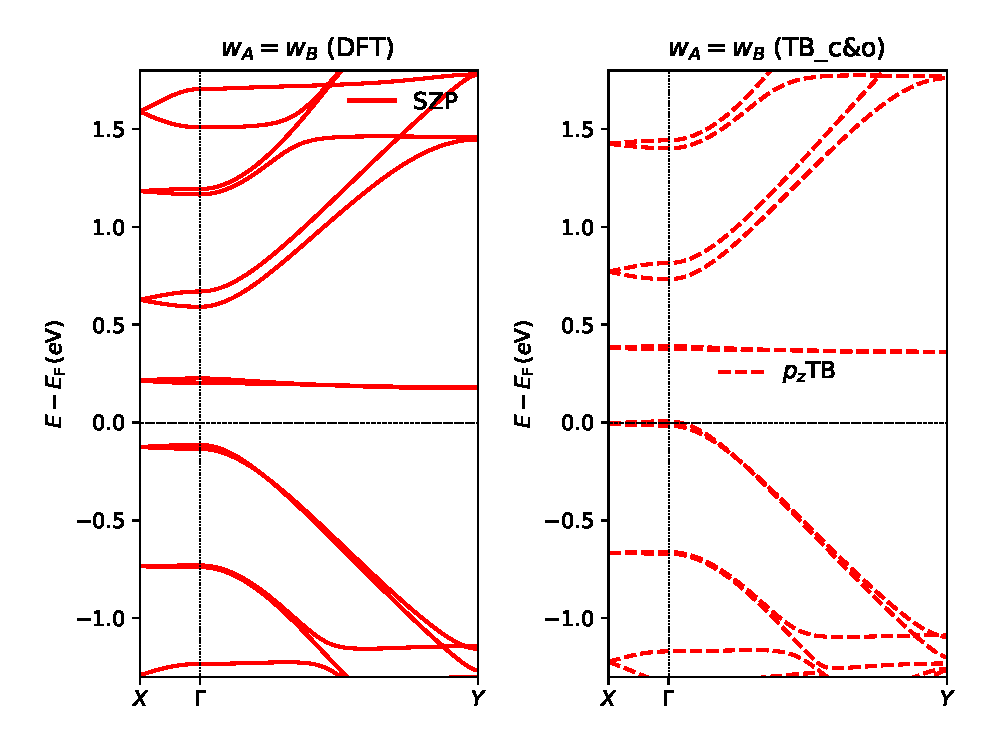
\includegraphics[width=\textwidth]{Figures/p_O4.eps}
    \end{subfigure}
    \vskip
    \hspace{50pt}
    \begin{subfigure}[b]{0.7\textwidth}
    \centering
    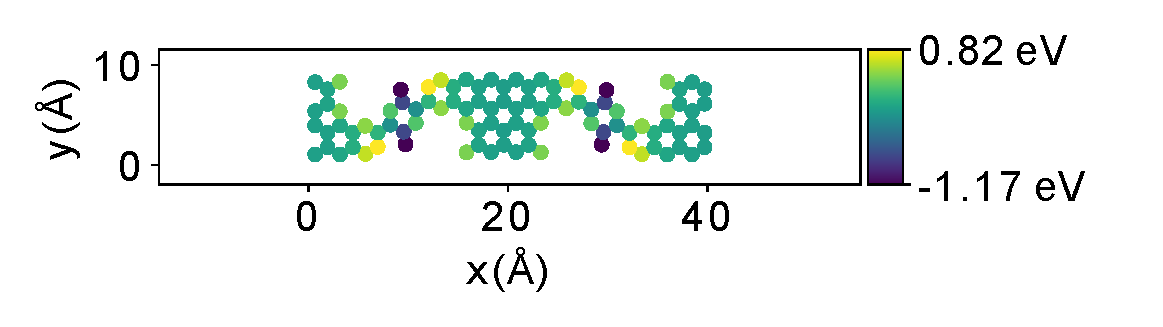
\includegraphics[width=\textwidth]{Figures/PS4O.eps}
    \end{subfigure}
    \vspace{-1\baselineskip}
    \caption{Figure showing the band structures obtained using DFT (above) and a potential map of the system (below)}
    \label{PS4O}
\end{figure}
Following, in \cref{PS4Odev} band plots obtained with the developed program is shown. Firstly a band plot without any changes to the on-site potential and next to it a band plot where the on-site potential of the added sites have been changed.
\begin{figure}[h]
    \centering
    \begin{subfigure}[b]{0.25\textwidth}
    \centering
    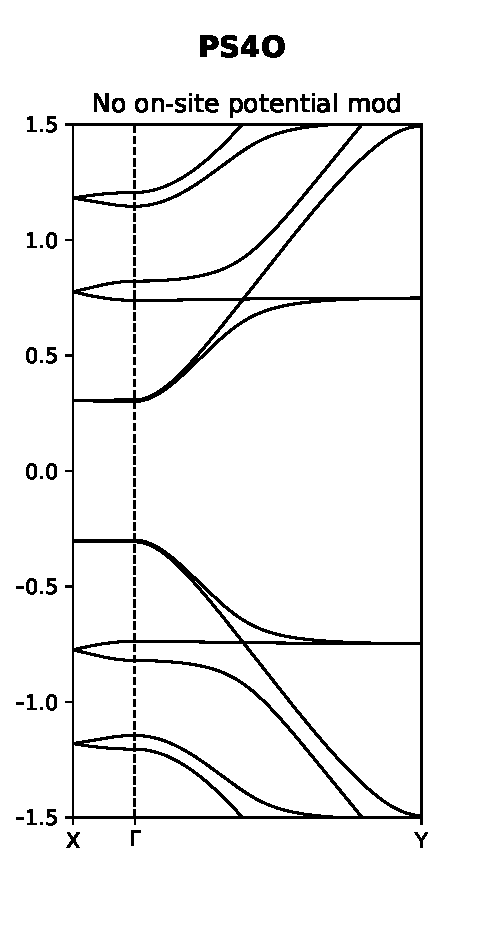
\includegraphics[width=\textwidth]{Figures/PS4Onomod.eps}
    \label{PS4Odevnomod}
    \end{subfigure}
    ~
    \begin{subfigure}[b]{0.25\textwidth}
    \centering
    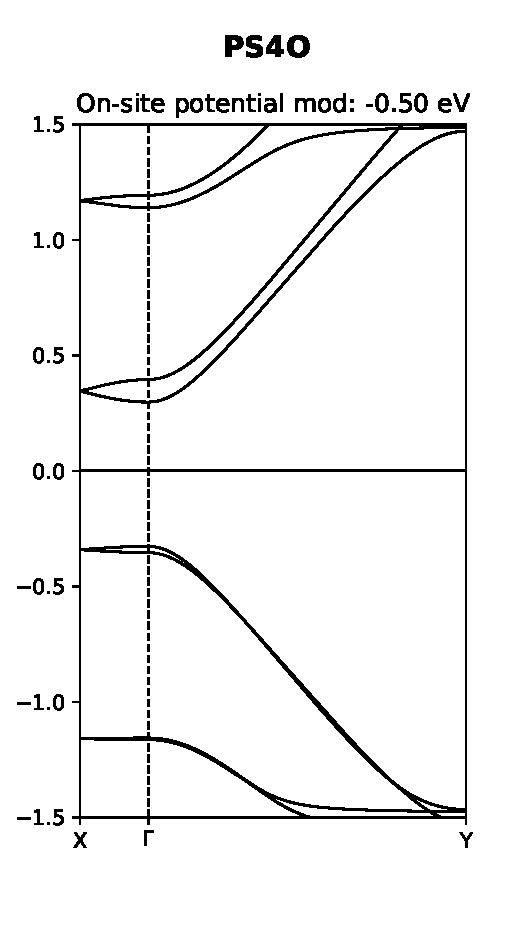
\includegraphics[width=\textwidth]{Figures/PS4Omod.eps}
    \label{PS4Odevmod}
    \end{subfigure}
    \vspace{-2\baselineskip}
    \caption{Figure showing band structures obtained using developed program. One with no on-site potential mods (left) and one with the on-site potential changed to \SI{-0.5}{\electronvolt} (right).} 
    \label{PS4Odev}
\end{figure}
as seen \cref{PS4Odevnomod} the band structure produced does not give the right result right away. This is because that the script assumes the same potential everywhere in the system. But as seen on the potential map in \cref{PS4O} especially the potential of the added sites (dark blue) are lower than the rest of the system. To compensate for this, the on-site potential values of those specific sites have been changed by \(\SI{-0.5}{\electronvolt}\) in the script (\cref{PS4Odevmod}) and the result is much closer to that in \cref{PS4O}.
\subsection{Test 2 simulating hydrogenation of para-NPG with added oxygen atoms}
Next test will be with the 'PS4OH' system. Again the basis structure is para-NPG with added oxygen, but here the aim is to simulate hydrogenation, so therefore the oxygen atoms added will become hydroxide groups. (see \cref{appfigs}, \cref{Strucow}, no. 6). Here the test is to show the difference between removing a OH site entirely (effectively the hydrogen in hydroxide removes the extra pi-electron in oxygen from the system, which can be simulated by removing the atoms entirely) and lowering the on-site potential of the oxygen in the OH group significantly in relation to the rest of the system. Again the results from DTF is shown first in \cref{PS4OH} and afterwards results from developed programs. 
\begin{figure}[h]
    \centering
    \begin{subfigure}[b]{0.5\textwidth}
    \centering
    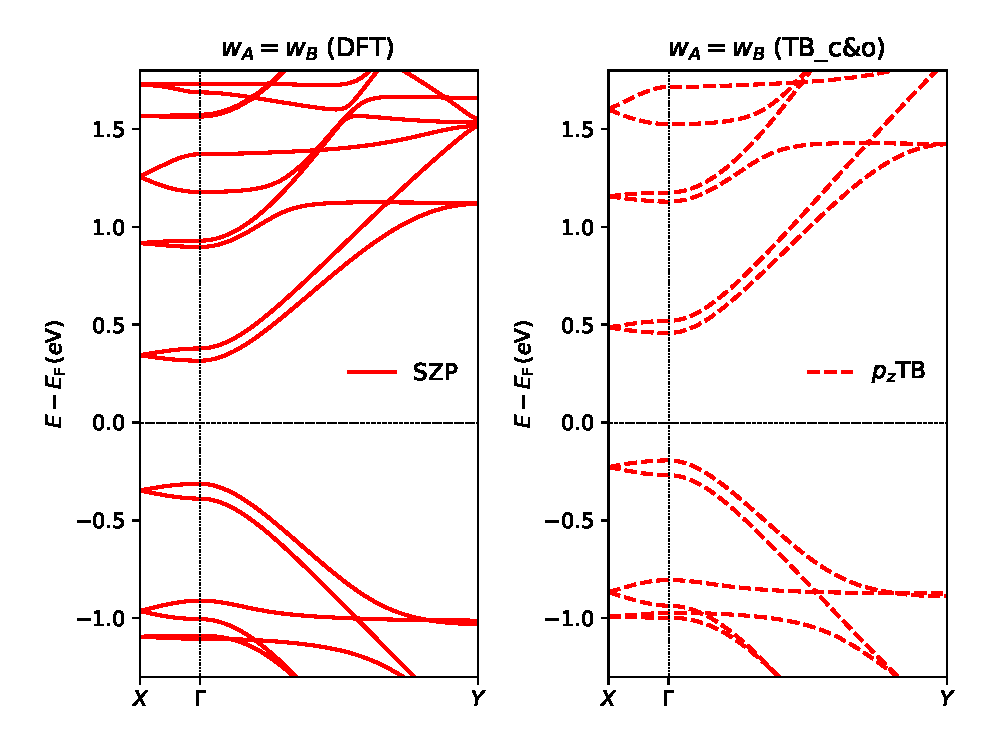
\includegraphics[width=\textwidth]{Figures/p_H4O4.eps}
    \end{subfigure}
    \vskip
    \hspace{50pt}
    \begin{subfigure}[b]{0.7\textwidth}
    \centering
    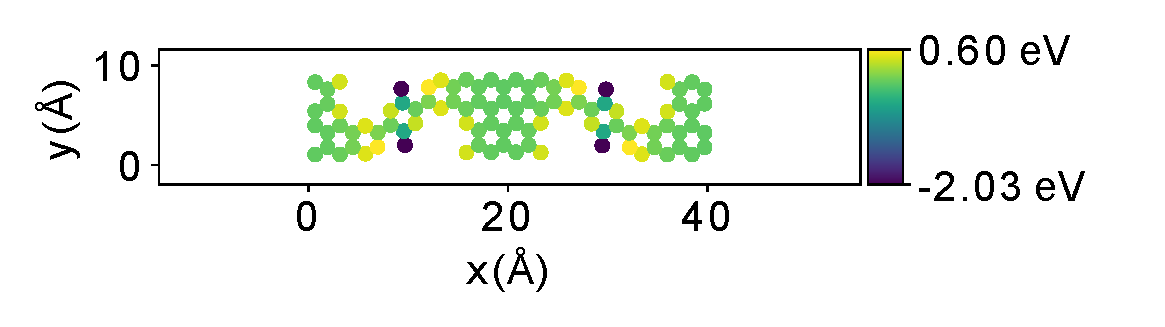
\includegraphics[width=\textwidth]{Figures/PS4OH.eps}
    \end{subfigure}
    \vspace{-1\baselineskip}
    \caption{Figure showing the band structures obtained using DFT (above) and a potential map of the system (below)}
    \label{PS4OH}
\end{figure}
Multiple on-site potentials as well as removal of the specific atomic sites were tested to see which one came closest to that of the band structures in \cref{PS4OH}. The removal was done by removing specific coordinates in the given files before it was run through the script. 
\begin{figure}[h]
    \centering
    \begin{subfigure}[b]{0.25\textwidth}
    \centering
    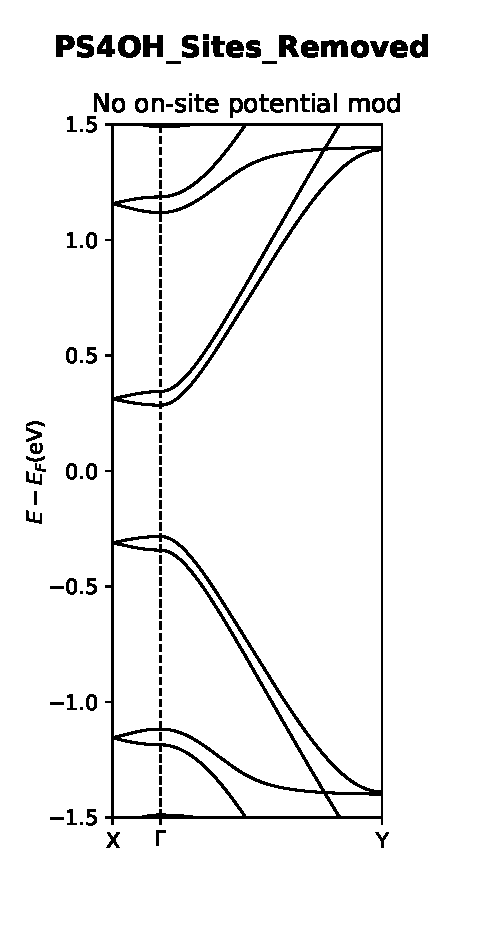
\includegraphics[width=\textwidth]{Figures/PS4OHSitesRemoved.eps}
    \label{PS4OHremove}
    \end{subfigure}
    ~
    \begin{subfigure}[b]{0.25\textwidth}
    \centering
    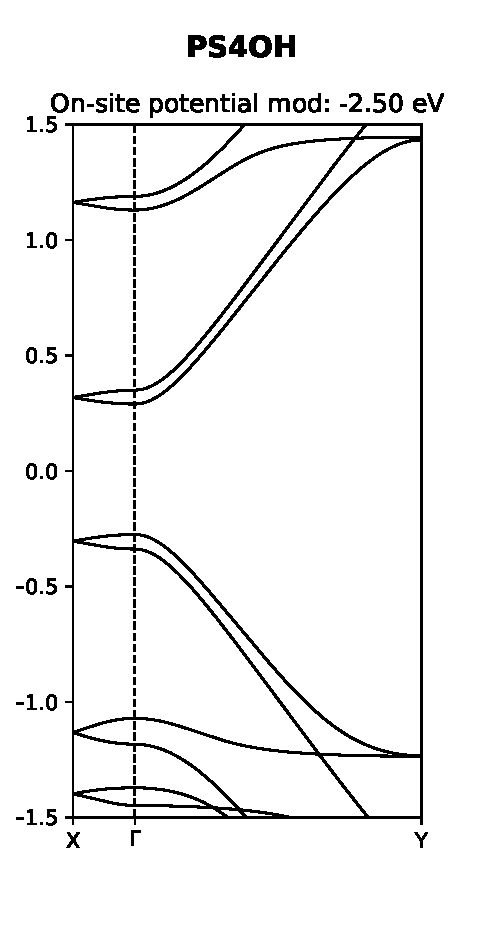
\includegraphics[width=\textwidth]{Figures/PS4OHmod1.eps}
    \label{PS4OHmod1}
    \end{subfigure}
    ~
    \begin{subfigure}[b]{0.25\textwidth}
    \centering
    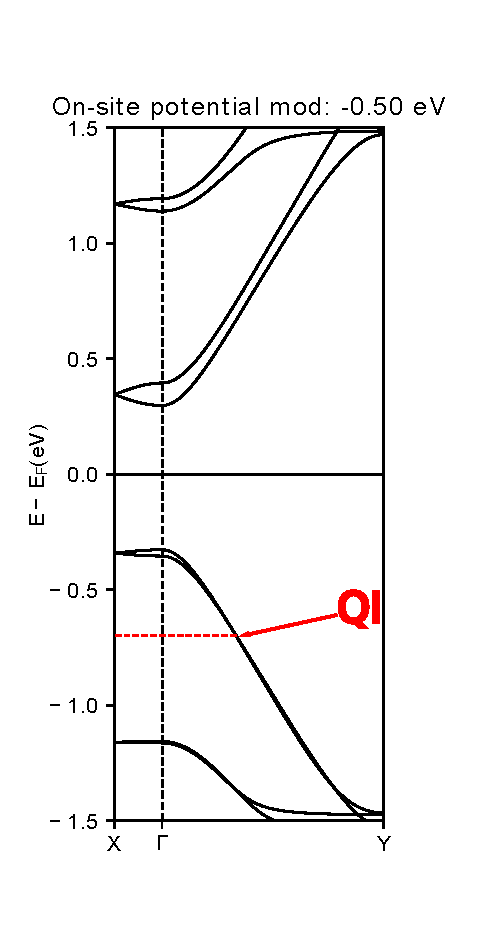
\includegraphics[width=\textwidth]{Figures/PS4OHmod2.eps}
    \label{PS4OHdevmod2}
    \end{subfigure}
    \vspace{-2\baselineskip}
    \caption{Figure showing band structures obtained using developed program. Left: band plot where the added sites have been removed, centre: band plot where the on-site potential has been changed by \(\SI{-2.5}{\electronvolt}\), right: band plot where the on-site potential has been changed by \(\SI{-2.0}{\electronvolt}\).} 
    \label{PS4OHdev}
\end{figure}
A seen in \cref{PS4OHremove} the effect of removing the sites gives a plot, somewhat in agreement with \cref{PS4OH}. However the lowest and highest bands does not show. The two other plots in \cref{PS4OHdev} show how gradually changing the on-site potential gets better and better agreement with DFTs. A on-site potential of \(\SI{-2.5}{\electronvolt}\) proved to be a bit too high, though still showing good agreement. Lowering the potential to \(\SI{-2.0}{\electronvolt}\) which is the value similar to that given by the lowest potential in the potential map \cref{PS4OH}, yielded a result that is pretty much spot on, considering the valence bands, when compared with DFT. 
\subsection{Test 3}
\subsection{Test 4}
\subsection{Test 5}
\subsection{Test 6}


\section{Discussion}\label{Disc}
\input{sections/Discussion.tex}
\section{Conclusion}\label{Conc}
%!TEX root = ../Main.tex
Concluding on section \cref{theorysec,hamilsec,greensec,transec}, simple numerical methods have been developed and implemented with success. The resulting LDOS, band and transmission plots, especially for NPG, show that the method indeed is capable of reproducing results from DFT and TBtrans calculation. However, there are small discrepancy in the results obtained when comparing with DFT. The reasons for the discrepancy is not immediately clear from the results but there might be a couple of things to point out and keep in mind. The method has been developed on the assumption that all atoms are in the plane and they, as a baseline all have the same potential. This might cause some of the small differences that one can see in the results, especially the transmission plots of \cref{transmissionplots}. So the DFT approach might have picked up some these effects that the developed method could not.\\
In \cref{testsec} the program showed that it too could reproduce results of much more complicated systems with multiple atom species, not just carbon. The initial results where not strongly resembling the DFT calculations, but after some tweaking of specific on-site potentials, the agreement became very good. This gave some valuable insights as to what happens chemically in NPG when it is functionalised with different atoms. These discoveries also made it more clear which flaws the method had and how to go about simulating even more complicated systems. One approach which should be implemented is automating the manipulation of the on-site potentials of species bonded to the bridges in NPG. The scripts used in this project only took into account the specific atoms bonded to the NPG and changed their potential. However, as one can see in potential maps in the figures of \cref{testsec}, the potential is not only changing at the specific sites where the atoms have bonded. It also changes the on-site potential of all the other atoms in the system. This was not accounted for in the developed method. However, there is a system as to how these potentials change. In future work, a possible way to account for the potential change, is to look at each carbon atom in the system, and count how many bonds it makes to other atoms. The amount of bonds the atom makes is, in part, determining its potential. By changing the potential relative to how many bonds they are making to other atoms, it would be possible to get a more precise picture of the potentials in the system and thus give an even more precise result when calculating band plots and transmission. \\
This proposal is for working out the details of producing the most accurate results possible. The main fact is that the project succeeded in making a program that could reproduce result that qualitatively was the same as the DFT, but in a much simpler way. This should pave the way for a method faster computing of all different kinds of NPG systems in a field that is still evolving rapidly. By showing a method where DFT has been avoided, it also gives value to the intuitive understanding of NPG systems which should make this field more available to a broader audience.  
\newpage
\begin{acknowledgments}
	The authors would like to thank...
\end{acknowledgments}
%End of text
% List of ToDos
%\listoftodos %Uncomment for list of todos
%Bibliography herunder:
%\newpage
\onecolumngrid
\bibliography{Bibliography}

\newpage
\listoffigures
\listoftables
\listoflistings
%\listoftodos
\newpage
%Appendicer herunder:
% !TEX root = Main.tex
\appendix
\appendixpage
\addappheadtotoc
\section{The benzene molecule}\label{benzex}
\begin{wrapfigure}[7]{r}{.3\textwidth}
	\vspace{-2.3em}
	\centering
	\begin{tikzpicture}
		\chemfig{1*6(-2-3-4-5-6-)}
	\end{tikzpicture}
	\caption{Indices of a benzene molecule}\label{benz}
\end{wrapfigure}
As an example the Hamiltonian of benzene is considered. In \cref{benz} one can see the indices of a benzene molecule. Remember that \(\bra{\phi_{\pi}(1)}\hat{H}\ket{\phi_{\pi}(1)} = 0\) and \cref{V}, the Hamiltonian reads:
\begin{align}
	\mqty{                            \\ \\ \\ \vb{H} = V_{pp\pi}\\ \\ \\} \ \mqty{						&  \mqty{1 & 2 & 3 & 4 & 5 & 6} \\
		\mqty{1                           \\ 2 \\ 3 \\ 4 \\ 5 \\ 6} &	\mqty*(0 & 1 & 0 & 0 & 0 & 1 \\
	1 & 0 & 1 & 0 & 0 & 0             \\
	0 & 1 & 0 & 1 & 0 & 0             \\
	0 & 0 & 1 & 0 & 1 & 0             \\
	0 & 0 & 0 & 1 & 0 & 1             \\
	1 & 0 & 0 & 0 & 1 & 0)}\label{BH}
\end{align}
As a helping aid, \cref{BH} shows the atomic indices of the atom on the top and to the left of the matrix. This will give an understanding of how to work with such matrices.
The structure of the benzene molecule is rotationally symmetric and rotating the indices one sixth must yield the same Hamiltonian. Consider the energy eigenvector:
\begin{align}
	\phi = \mqty(c_1 & c_2 & c_3 & c_4 & c_5 & c_6)
\end{align}
There must exist an operator that rotates the indices as such:
\begin{align}
	C_6\phi = \mqty(c_2 & c_3 & c_4 & c_5 & c_6 & c_1)
\end{align}
The rotated Hamiltonian is the same, and thus \(C_6\) and \(\vb{H}\) commute. The rotated vector must be an eigenvector with the same energy and it should be possible to find simultaneous eigenvectors to \(C_6\) and \(\vb{H}\).
\begin{align}
	C_6\phi = \mqty(c_2 & c_3 & c_4 & c_5 & c_6 & c_1) = \lambda\mqty(c_1 & c_2 & c_3 & c_4 & c_5 & c_6)
\end{align}
This operator \(C_6\) is represented with the matrix:
\begin{align}
	\vb{C}_6 = \mqty*(0 & 1 & 0 & 0 & 0 & 0  \\
	0                   & 0 & 1 & 0 & 0 & 0  \\
	0                   & 0 & 0 & 1 & 0 & 0  \\
	0                   & 0 & 0 & 0 & 1 & 0  \\
	0                   & 0 & 0 & 0 & 0 & 1  \\
	1                   & 0 & 0 & 0 & 0 & 0)
\end{align}
It can quickly be shown that the normalised eigenvectors to \(C_6\) are
\begin{align}
	\phi_n = \frac{1}{\sqrt{6}}\mqty(\lambda_n^0 & \lambda_n^1 & \lambda_n^2 & \lambda_n^3 & \lambda_n^4 & \lambda_n^5), \quad \lambda_n = \exp{-i2\pi n / 6}, \quad n = 0,1,2,3,4,5
\end{align}
These eigenvectors are also eigenvectors for \(\vb{H}\) with the eigenvalues:
\begin{align}
	\varepsilon_n = \lambda_n + \lambda_{n-1} = 2 \cos{n\pi/3}
\end{align}
Thus thanks to the rotational symmetry it was possible to find the eigenvectors and eigenenergies for the Hamiltonian.
\section{Additional figures}\label{appfigs}
\begin{figure}[h]
	\centering
	\begin{subfigure}[b]{0.45\textwidth}
		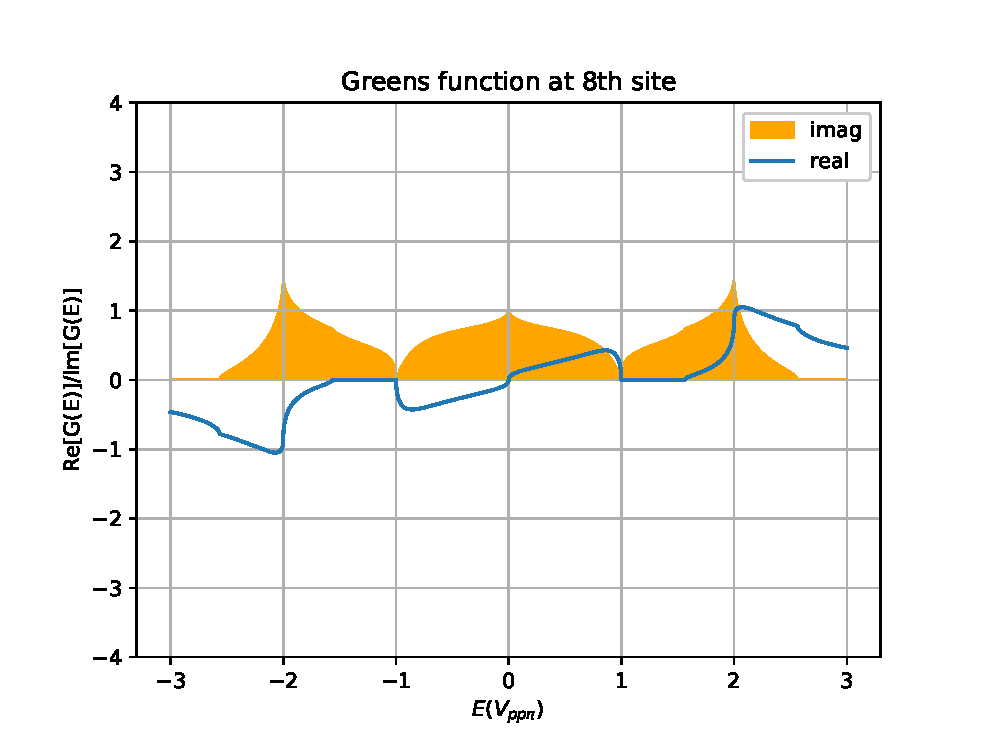
\includegraphics[width=\textwidth]{Figures/BetaimrealTE8.eps}
		\caption{Figure showing a plot of the Green's function at the \nth{8} site}
		\label{4th}
	\end{subfigure}
	~ %add desired spacing between images, e. g. ~, \quad, \qquad, \hfill etc.
	%(or a blank line to force the subfigure onto a new line)
	\begin{subfigure}[b]{0.45\textwidth}
		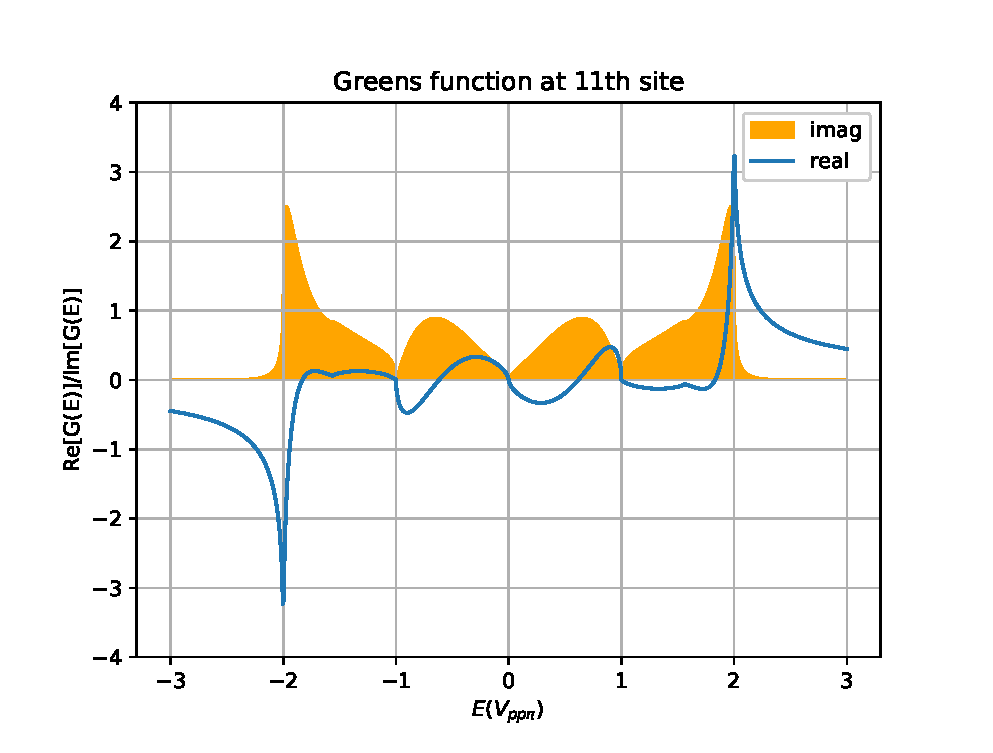
\includegraphics[width=\textwidth]{Figures/BetaimrealTE11.eps}
		\caption{Figure showing a plot of the Green's function at the \nth{11} site}
		\label{7th}
	\end{subfigure}
	\caption{Two plots showing how the Green's function changes as the site is changed. The \nth{8} and \nth{11} sites are corresponding to atoms of those indices (8, 11) in \cref{pointplot}. Note how the LDOS changes (imaginary part) for the different sites.}\label{siteLDOSplot}
\end{figure}
\begin{figure}[h]
	\centering
	\begin{subfigure}[b]{0.3\textwidth}
		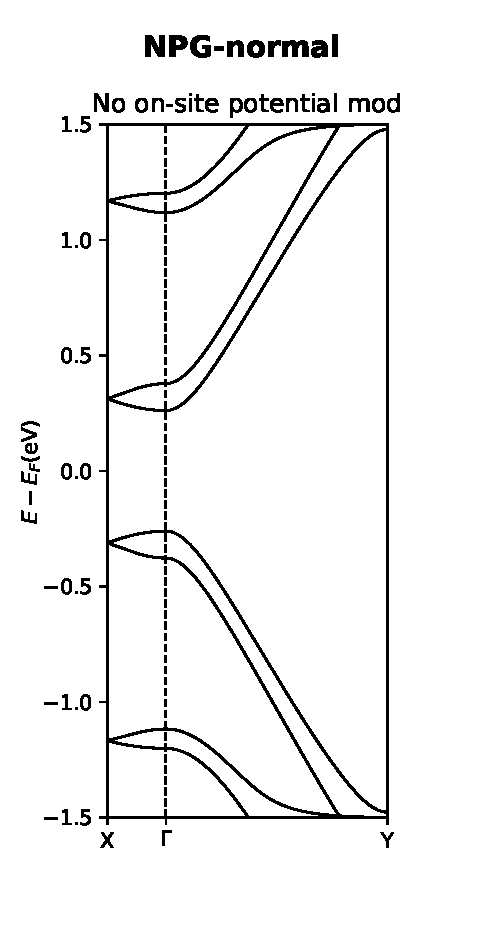
\includegraphics[width=\textwidth]{Figures/FabNPGBS.eps}
		\caption{Normal NPG}
		\label{Fabbs}
	\end{subfigure}
	~ %add desired spacing between images, e. g. ~, \quad, \qquad, \hfill etc.
	%(or a blank line to force the subfigure onto a new line)
	\begin{subfigure}[b]{0.3\textwidth}
		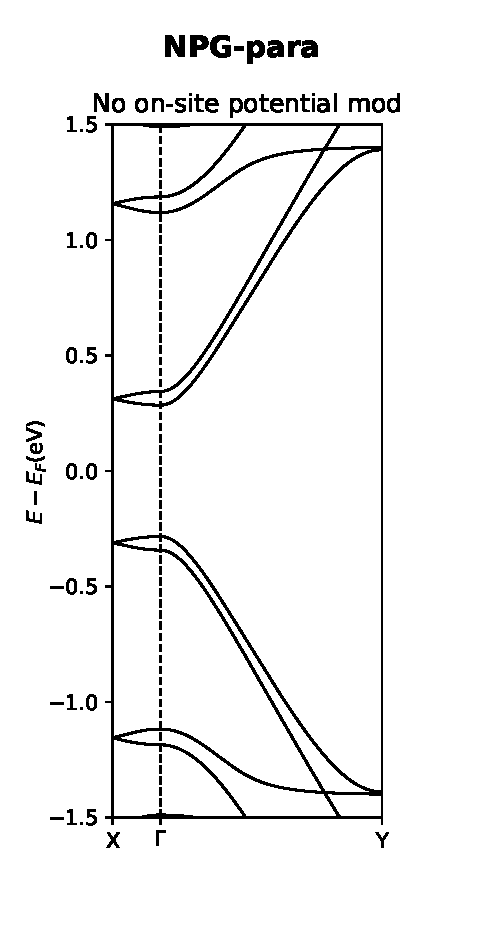
\includegraphics[width=\textwidth]{Figures/paraNPGBS.eps}
		\caption{Para NPG}
		\label{parabs}
	\end{subfigure}
	~ %add desired spacing between images, e. g. ~, \quad, \qquad, \hfill etc.
	%(or a blank line to force the subfigure onto a new line)
	\begin{subfigure}[b]{0.3\textwidth}
		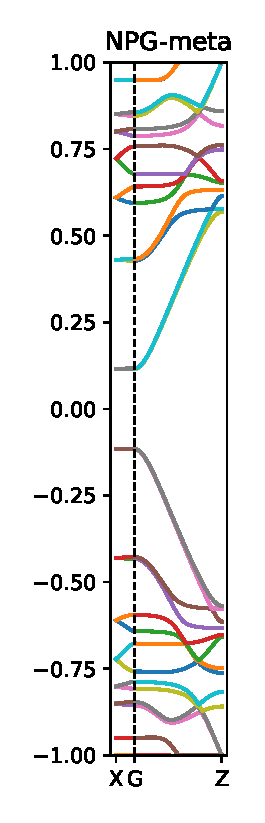
\includegraphics[width=\textwidth]{Figures/metaNPGBS.eps}
		\caption{Meta NPG}
		\label{metabs}
	\end{subfigure}
	\caption{Plot showing band structures in the energy range \SI{-1.5}{\electronvolt} to \SI{1.5}{\electronvolt} for normal, para and meta NPG. The are plotted between symmetry points \(X\) and \(Y\) with respect to the origin \(\Gamma\)}\label{allbands}
\end{figure}

\im{Listings/Functions.py}{245}{252}
\vspace{-1\baselineskip}
\captionof{listing}{Code piece showing how the periodic Hamiltonian, shifted in the transverse direction i created using the given unit vector in the y direction.}{\label{periodichamilcode}}\vspace{\baselineskip}

\im{Listings/Functions.py}{234}{242}
\vspace{-1\baselineskip}
\captionof{listing}{Code piece showing how the transmission per energy point, using equation \cref{transeq}}{\label{transmissioncode}\vspace{\baselineskip}

\newpage
\im{Listings/Functions.py}{237}{245}
\im{Listings/Functions.py}{72}{81}
\im{Listings/Functions.py}{84}{111}
\im{Listings/Functions.py}{198}{234}
% \section{Project overview}
% A Gantt chart is provided on the next page. \textbf{Not Updated.}
% \newpage
% \begin{turnpage}
% \setcounter{myWeekNum}{6}
% \ganttset{%
% 	calendar week text={\myWeek{}}%
% }
% \begin{figure}\vspace{-10mm}
% \begin{ganttchart}[
% 		hgrid,
% 		vgrid={*{6}{draw=none}, dotted},
% 		x unit=.15cm,
% 		%	y unit title=.6cm,
% 		%	y unit chart=.6cm,
% 		inline,
% 		milestone inline label node/.append style={left=5mm},
% 		milestone/.append style={xscale=3},
% 		time slot format=isodate,
% 		time slot format/start date=2019-02-04
% 	]{2019-02-04}{2019-05-31}
% 	\gantttitlecalendar{year, month=shortname, week}\\
% 	\ganttgroup{Report writing}{2019-02-25}{2019-05-31}\\
% 	\ganttgroup[inline = false]{Course 33442}{2019-02-04}{2019-03-31}\\
% 	\ganttbar{Ch. 1 \& 2}{2019-02-04}{2019-02-17}\\
% 	\ganttlinkedbar[link bulge=2]{Ch. 3}{2019-02-18}{2019-02-24}\\
% 	\ganttlinkedbar[link bulge=2,bar inline label node/.style={right=15pt}]{Ch. 4 \& 5}{2019-02-25}{2019-03-03}\\
% 	\ganttgroup[inline = false]{Python code}{2019-03-04}{2019-03-31}\\
% 	\ganttbar{Py TB scripts}{2019-02-18}{2019-03-17}\\
% 	\ganttlinkedbar[link bulge=2, bar inline label node/.style={right=45pt}]{Small NPG systems simulations}{2019-03-10}{2019-03-31}\\
% 	\ganttmilestone{Proof of Concept with Python}{2019-03-31}\\
% 	\ganttgroup[inline = false]{Large scale TB}{2019-04-01}{2019-04-28}\\
% 	\ganttbar[bar inline label node/.style={left=10pt}]{SISL \& TBtrans tutorial}{2019-04-01}{2019-04-05}\\
% 	\ganttlinkedbar[link bulge=2, bar inline label node/.style={right=50pt}]{Setup NPG variations}{2019-04-06}{2019-04-28}\\
% 	\ganttgroup[inline = false]{Generate data}{2019-04-28}{2019-05-31}\\
% 	\ganttmilestone{Hand in report}{2019-05-31}
% \end{ganttchart}
% \end{figure}
% \end{turnpage}
% \clearpage
% \global\pdfpageattr\expandafter{\the\pdfpageattr/Rotate 90}

\end{document}
